
% Default to the notebook output style

    


% Inherit from the specified cell style.




    
\documentclass[11pt]{article}

    
    
    \usepackage[T1]{fontenc}
    % Nicer default font (+ math font) than Computer Modern for most use cases
    \usepackage{mathpazo}

    % Basic figure setup, for now with no caption control since it's done
    % automatically by Pandoc (which extracts ![](path) syntax from Markdown).
    \usepackage{graphicx}
    % We will generate all images so they have a width \maxwidth. This means
    % that they will get their normal width if they fit onto the page, but
    % are scaled down if they would overflow the margins.
    \makeatletter
    \def\maxwidth{\ifdim\Gin@nat@width>\linewidth\linewidth
    \else\Gin@nat@width\fi}
    \makeatother
    \let\Oldincludegraphics\includegraphics
    % Set max figure width to be 80% of text width, for now hardcoded.
    \renewcommand{\includegraphics}[1]{\Oldincludegraphics[width=.8\maxwidth]{#1}}
    % Ensure that by default, figures have no caption (until we provide a
    % proper Figure object with a Caption API and a way to capture that
    % in the conversion process - todo).
    \usepackage{caption}
    \DeclareCaptionLabelFormat{nolabel}{}
    \captionsetup{labelformat=nolabel}

    \usepackage{adjustbox} % Used to constrain images to a maximum size 
    \usepackage{xcolor} % Allow colors to be defined
    \usepackage{enumerate} % Needed for markdown enumerations to work
    \usepackage{geometry} % Used to adjust the document margins
    \usepackage{amsmath} % Equations
    \usepackage{amssymb} % Equations
    \usepackage{textcomp} % defines textquotesingle
    % Hack from http://tex.stackexchange.com/a/47451/13684:
    \AtBeginDocument{%
        \def\PYZsq{\textquotesingle}% Upright quotes in Pygmentized code
    }
    \usepackage{upquote} % Upright quotes for verbatim code
    \usepackage{eurosym} % defines \euro
    \usepackage[mathletters]{ucs} % Extended unicode (utf-8) support
    \usepackage[utf8x]{inputenc} % Allow utf-8 characters in the tex document
    \usepackage{fancyvrb} % verbatim replacement that allows latex
    \usepackage{grffile} % extends the file name processing of package graphics 
                         % to support a larger range 
    % The hyperref package gives us a pdf with properly built
    % internal navigation ('pdf bookmarks' for the table of contents,
    % internal cross-reference links, web links for URLs, etc.)
    \usepackage{hyperref}
    \usepackage{longtable} % longtable support required by pandoc >1.10
    \usepackage{booktabs}  % table support for pandoc > 1.12.2
    \usepackage[inline]{enumitem} % IRkernel/repr support (it uses the enumerate* environment)
    \usepackage[normalem]{ulem} % ulem is needed to support strikethroughs (\sout)
                                % normalem makes italics be italics, not underlines
    

    
    
    % Colors for the hyperref package
    \definecolor{urlcolor}{rgb}{0,.145,.698}
    \definecolor{linkcolor}{rgb}{.71,0.21,0.01}
    \definecolor{citecolor}{rgb}{.12,.54,.11}

    % ANSI colors
    \definecolor{ansi-black}{HTML}{3E424D}
    \definecolor{ansi-black-intense}{HTML}{282C36}
    \definecolor{ansi-red}{HTML}{E75C58}
    \definecolor{ansi-red-intense}{HTML}{B22B31}
    \definecolor{ansi-green}{HTML}{00A250}
    \definecolor{ansi-green-intense}{HTML}{007427}
    \definecolor{ansi-yellow}{HTML}{DDB62B}
    \definecolor{ansi-yellow-intense}{HTML}{B27D12}
    \definecolor{ansi-blue}{HTML}{208FFB}
    \definecolor{ansi-blue-intense}{HTML}{0065CA}
    \definecolor{ansi-magenta}{HTML}{D160C4}
    \definecolor{ansi-magenta-intense}{HTML}{A03196}
    \definecolor{ansi-cyan}{HTML}{60C6C8}
    \definecolor{ansi-cyan-intense}{HTML}{258F8F}
    \definecolor{ansi-white}{HTML}{C5C1B4}
    \definecolor{ansi-white-intense}{HTML}{A1A6B2}

    % commands and environments needed by pandoc snippets
    % extracted from the output of `pandoc -s`
    \providecommand{\tightlist}{%
      \setlength{\itemsep}{0pt}\setlength{\parskip}{0pt}}
    \DefineVerbatimEnvironment{Highlighting}{Verbatim}{commandchars=\\\{\}}
    % Add ',fontsize=\small' for more characters per line
    \newenvironment{Shaded}{}{}
    \newcommand{\KeywordTok}[1]{\textcolor[rgb]{0.00,0.44,0.13}{\textbf{{#1}}}}
    \newcommand{\DataTypeTok}[1]{\textcolor[rgb]{0.56,0.13,0.00}{{#1}}}
    \newcommand{\DecValTok}[1]{\textcolor[rgb]{0.25,0.63,0.44}{{#1}}}
    \newcommand{\BaseNTok}[1]{\textcolor[rgb]{0.25,0.63,0.44}{{#1}}}
    \newcommand{\FloatTok}[1]{\textcolor[rgb]{0.25,0.63,0.44}{{#1}}}
    \newcommand{\CharTok}[1]{\textcolor[rgb]{0.25,0.44,0.63}{{#1}}}
    \newcommand{\StringTok}[1]{\textcolor[rgb]{0.25,0.44,0.63}{{#1}}}
    \newcommand{\CommentTok}[1]{\textcolor[rgb]{0.38,0.63,0.69}{\textit{{#1}}}}
    \newcommand{\OtherTok}[1]{\textcolor[rgb]{0.00,0.44,0.13}{{#1}}}
    \newcommand{\AlertTok}[1]{\textcolor[rgb]{1.00,0.00,0.00}{\textbf{{#1}}}}
    \newcommand{\FunctionTok}[1]{\textcolor[rgb]{0.02,0.16,0.49}{{#1}}}
    \newcommand{\RegionMarkerTok}[1]{{#1}}
    \newcommand{\ErrorTok}[1]{\textcolor[rgb]{1.00,0.00,0.00}{\textbf{{#1}}}}
    \newcommand{\NormalTok}[1]{{#1}}
    
    % Additional commands for more recent versions of Pandoc
    \newcommand{\ConstantTok}[1]{\textcolor[rgb]{0.53,0.00,0.00}{{#1}}}
    \newcommand{\SpecialCharTok}[1]{\textcolor[rgb]{0.25,0.44,0.63}{{#1}}}
    \newcommand{\VerbatimStringTok}[1]{\textcolor[rgb]{0.25,0.44,0.63}{{#1}}}
    \newcommand{\SpecialStringTok}[1]{\textcolor[rgb]{0.73,0.40,0.53}{{#1}}}
    \newcommand{\ImportTok}[1]{{#1}}
    \newcommand{\DocumentationTok}[1]{\textcolor[rgb]{0.73,0.13,0.13}{\textit{{#1}}}}
    \newcommand{\AnnotationTok}[1]{\textcolor[rgb]{0.38,0.63,0.69}{\textbf{\textit{{#1}}}}}
    \newcommand{\CommentVarTok}[1]{\textcolor[rgb]{0.38,0.63,0.69}{\textbf{\textit{{#1}}}}}
    \newcommand{\VariableTok}[1]{\textcolor[rgb]{0.10,0.09,0.49}{{#1}}}
    \newcommand{\ControlFlowTok}[1]{\textcolor[rgb]{0.00,0.44,0.13}{\textbf{{#1}}}}
    \newcommand{\OperatorTok}[1]{\textcolor[rgb]{0.40,0.40,0.40}{{#1}}}
    \newcommand{\BuiltInTok}[1]{{#1}}
    \newcommand{\ExtensionTok}[1]{{#1}}
    \newcommand{\PreprocessorTok}[1]{\textcolor[rgb]{0.74,0.48,0.00}{{#1}}}
    \newcommand{\AttributeTok}[1]{\textcolor[rgb]{0.49,0.56,0.16}{{#1}}}
    \newcommand{\InformationTok}[1]{\textcolor[rgb]{0.38,0.63,0.69}{\textbf{\textit{{#1}}}}}
    \newcommand{\WarningTok}[1]{\textcolor[rgb]{0.38,0.63,0.69}{\textbf{\textit{{#1}}}}}
    
    
    % Define a nice break command that doesn't care if a line doesn't already
    % exist.
    \def\br{\hspace*{\fill} \\* }
    % Math Jax compatability definitions
    \def\gt{>}
    \def\lt{<}
    % Document parameters
    \title{Bayesian Inference in Larger Models}
    
    
    

    % Pygments definitions
    
\makeatletter
\def\PY@reset{\let\PY@it=\relax \let\PY@bf=\relax%
    \let\PY@ul=\relax \let\PY@tc=\relax%
    \let\PY@bc=\relax \let\PY@ff=\relax}
\def\PY@tok#1{\csname PY@tok@#1\endcsname}
\def\PY@toks#1+{\ifx\relax#1\empty\else%
    \PY@tok{#1}\expandafter\PY@toks\fi}
\def\PY@do#1{\PY@bc{\PY@tc{\PY@ul{%
    \PY@it{\PY@bf{\PY@ff{#1}}}}}}}
\def\PY#1#2{\PY@reset\PY@toks#1+\relax+\PY@do{#2}}

\expandafter\def\csname PY@tok@w\endcsname{\def\PY@tc##1{\textcolor[rgb]{0.73,0.73,0.73}{##1}}}
\expandafter\def\csname PY@tok@c\endcsname{\let\PY@it=\textit\def\PY@tc##1{\textcolor[rgb]{0.25,0.50,0.50}{##1}}}
\expandafter\def\csname PY@tok@cp\endcsname{\def\PY@tc##1{\textcolor[rgb]{0.74,0.48,0.00}{##1}}}
\expandafter\def\csname PY@tok@k\endcsname{\let\PY@bf=\textbf\def\PY@tc##1{\textcolor[rgb]{0.00,0.50,0.00}{##1}}}
\expandafter\def\csname PY@tok@kp\endcsname{\def\PY@tc##1{\textcolor[rgb]{0.00,0.50,0.00}{##1}}}
\expandafter\def\csname PY@tok@kt\endcsname{\def\PY@tc##1{\textcolor[rgb]{0.69,0.00,0.25}{##1}}}
\expandafter\def\csname PY@tok@o\endcsname{\def\PY@tc##1{\textcolor[rgb]{0.40,0.40,0.40}{##1}}}
\expandafter\def\csname PY@tok@ow\endcsname{\let\PY@bf=\textbf\def\PY@tc##1{\textcolor[rgb]{0.67,0.13,1.00}{##1}}}
\expandafter\def\csname PY@tok@nb\endcsname{\def\PY@tc##1{\textcolor[rgb]{0.00,0.50,0.00}{##1}}}
\expandafter\def\csname PY@tok@nf\endcsname{\def\PY@tc##1{\textcolor[rgb]{0.00,0.00,1.00}{##1}}}
\expandafter\def\csname PY@tok@nc\endcsname{\let\PY@bf=\textbf\def\PY@tc##1{\textcolor[rgb]{0.00,0.00,1.00}{##1}}}
\expandafter\def\csname PY@tok@nn\endcsname{\let\PY@bf=\textbf\def\PY@tc##1{\textcolor[rgb]{0.00,0.00,1.00}{##1}}}
\expandafter\def\csname PY@tok@ne\endcsname{\let\PY@bf=\textbf\def\PY@tc##1{\textcolor[rgb]{0.82,0.25,0.23}{##1}}}
\expandafter\def\csname PY@tok@nv\endcsname{\def\PY@tc##1{\textcolor[rgb]{0.10,0.09,0.49}{##1}}}
\expandafter\def\csname PY@tok@no\endcsname{\def\PY@tc##1{\textcolor[rgb]{0.53,0.00,0.00}{##1}}}
\expandafter\def\csname PY@tok@nl\endcsname{\def\PY@tc##1{\textcolor[rgb]{0.63,0.63,0.00}{##1}}}
\expandafter\def\csname PY@tok@ni\endcsname{\let\PY@bf=\textbf\def\PY@tc##1{\textcolor[rgb]{0.60,0.60,0.60}{##1}}}
\expandafter\def\csname PY@tok@na\endcsname{\def\PY@tc##1{\textcolor[rgb]{0.49,0.56,0.16}{##1}}}
\expandafter\def\csname PY@tok@nt\endcsname{\let\PY@bf=\textbf\def\PY@tc##1{\textcolor[rgb]{0.00,0.50,0.00}{##1}}}
\expandafter\def\csname PY@tok@nd\endcsname{\def\PY@tc##1{\textcolor[rgb]{0.67,0.13,1.00}{##1}}}
\expandafter\def\csname PY@tok@s\endcsname{\def\PY@tc##1{\textcolor[rgb]{0.73,0.13,0.13}{##1}}}
\expandafter\def\csname PY@tok@sd\endcsname{\let\PY@it=\textit\def\PY@tc##1{\textcolor[rgb]{0.73,0.13,0.13}{##1}}}
\expandafter\def\csname PY@tok@si\endcsname{\let\PY@bf=\textbf\def\PY@tc##1{\textcolor[rgb]{0.73,0.40,0.53}{##1}}}
\expandafter\def\csname PY@tok@se\endcsname{\let\PY@bf=\textbf\def\PY@tc##1{\textcolor[rgb]{0.73,0.40,0.13}{##1}}}
\expandafter\def\csname PY@tok@sr\endcsname{\def\PY@tc##1{\textcolor[rgb]{0.73,0.40,0.53}{##1}}}
\expandafter\def\csname PY@tok@ss\endcsname{\def\PY@tc##1{\textcolor[rgb]{0.10,0.09,0.49}{##1}}}
\expandafter\def\csname PY@tok@sx\endcsname{\def\PY@tc##1{\textcolor[rgb]{0.00,0.50,0.00}{##1}}}
\expandafter\def\csname PY@tok@m\endcsname{\def\PY@tc##1{\textcolor[rgb]{0.40,0.40,0.40}{##1}}}
\expandafter\def\csname PY@tok@gh\endcsname{\let\PY@bf=\textbf\def\PY@tc##1{\textcolor[rgb]{0.00,0.00,0.50}{##1}}}
\expandafter\def\csname PY@tok@gu\endcsname{\let\PY@bf=\textbf\def\PY@tc##1{\textcolor[rgb]{0.50,0.00,0.50}{##1}}}
\expandafter\def\csname PY@tok@gd\endcsname{\def\PY@tc##1{\textcolor[rgb]{0.63,0.00,0.00}{##1}}}
\expandafter\def\csname PY@tok@gi\endcsname{\def\PY@tc##1{\textcolor[rgb]{0.00,0.63,0.00}{##1}}}
\expandafter\def\csname PY@tok@gr\endcsname{\def\PY@tc##1{\textcolor[rgb]{1.00,0.00,0.00}{##1}}}
\expandafter\def\csname PY@tok@ge\endcsname{\let\PY@it=\textit}
\expandafter\def\csname PY@tok@gs\endcsname{\let\PY@bf=\textbf}
\expandafter\def\csname PY@tok@gp\endcsname{\let\PY@bf=\textbf\def\PY@tc##1{\textcolor[rgb]{0.00,0.00,0.50}{##1}}}
\expandafter\def\csname PY@tok@go\endcsname{\def\PY@tc##1{\textcolor[rgb]{0.53,0.53,0.53}{##1}}}
\expandafter\def\csname PY@tok@gt\endcsname{\def\PY@tc##1{\textcolor[rgb]{0.00,0.27,0.87}{##1}}}
\expandafter\def\csname PY@tok@err\endcsname{\def\PY@bc##1{\setlength{\fboxsep}{0pt}\fcolorbox[rgb]{1.00,0.00,0.00}{1,1,1}{\strut ##1}}}
\expandafter\def\csname PY@tok@kc\endcsname{\let\PY@bf=\textbf\def\PY@tc##1{\textcolor[rgb]{0.00,0.50,0.00}{##1}}}
\expandafter\def\csname PY@tok@kd\endcsname{\let\PY@bf=\textbf\def\PY@tc##1{\textcolor[rgb]{0.00,0.50,0.00}{##1}}}
\expandafter\def\csname PY@tok@kn\endcsname{\let\PY@bf=\textbf\def\PY@tc##1{\textcolor[rgb]{0.00,0.50,0.00}{##1}}}
\expandafter\def\csname PY@tok@kr\endcsname{\let\PY@bf=\textbf\def\PY@tc##1{\textcolor[rgb]{0.00,0.50,0.00}{##1}}}
\expandafter\def\csname PY@tok@bp\endcsname{\def\PY@tc##1{\textcolor[rgb]{0.00,0.50,0.00}{##1}}}
\expandafter\def\csname PY@tok@fm\endcsname{\def\PY@tc##1{\textcolor[rgb]{0.00,0.00,1.00}{##1}}}
\expandafter\def\csname PY@tok@vc\endcsname{\def\PY@tc##1{\textcolor[rgb]{0.10,0.09,0.49}{##1}}}
\expandafter\def\csname PY@tok@vg\endcsname{\def\PY@tc##1{\textcolor[rgb]{0.10,0.09,0.49}{##1}}}
\expandafter\def\csname PY@tok@vi\endcsname{\def\PY@tc##1{\textcolor[rgb]{0.10,0.09,0.49}{##1}}}
\expandafter\def\csname PY@tok@vm\endcsname{\def\PY@tc##1{\textcolor[rgb]{0.10,0.09,0.49}{##1}}}
\expandafter\def\csname PY@tok@sa\endcsname{\def\PY@tc##1{\textcolor[rgb]{0.73,0.13,0.13}{##1}}}
\expandafter\def\csname PY@tok@sb\endcsname{\def\PY@tc##1{\textcolor[rgb]{0.73,0.13,0.13}{##1}}}
\expandafter\def\csname PY@tok@sc\endcsname{\def\PY@tc##1{\textcolor[rgb]{0.73,0.13,0.13}{##1}}}
\expandafter\def\csname PY@tok@dl\endcsname{\def\PY@tc##1{\textcolor[rgb]{0.73,0.13,0.13}{##1}}}
\expandafter\def\csname PY@tok@s2\endcsname{\def\PY@tc##1{\textcolor[rgb]{0.73,0.13,0.13}{##1}}}
\expandafter\def\csname PY@tok@sh\endcsname{\def\PY@tc##1{\textcolor[rgb]{0.73,0.13,0.13}{##1}}}
\expandafter\def\csname PY@tok@s1\endcsname{\def\PY@tc##1{\textcolor[rgb]{0.73,0.13,0.13}{##1}}}
\expandafter\def\csname PY@tok@mb\endcsname{\def\PY@tc##1{\textcolor[rgb]{0.40,0.40,0.40}{##1}}}
\expandafter\def\csname PY@tok@mf\endcsname{\def\PY@tc##1{\textcolor[rgb]{0.40,0.40,0.40}{##1}}}
\expandafter\def\csname PY@tok@mh\endcsname{\def\PY@tc##1{\textcolor[rgb]{0.40,0.40,0.40}{##1}}}
\expandafter\def\csname PY@tok@mi\endcsname{\def\PY@tc##1{\textcolor[rgb]{0.40,0.40,0.40}{##1}}}
\expandafter\def\csname PY@tok@il\endcsname{\def\PY@tc##1{\textcolor[rgb]{0.40,0.40,0.40}{##1}}}
\expandafter\def\csname PY@tok@mo\endcsname{\def\PY@tc##1{\textcolor[rgb]{0.40,0.40,0.40}{##1}}}
\expandafter\def\csname PY@tok@ch\endcsname{\let\PY@it=\textit\def\PY@tc##1{\textcolor[rgb]{0.25,0.50,0.50}{##1}}}
\expandafter\def\csname PY@tok@cm\endcsname{\let\PY@it=\textit\def\PY@tc##1{\textcolor[rgb]{0.25,0.50,0.50}{##1}}}
\expandafter\def\csname PY@tok@cpf\endcsname{\let\PY@it=\textit\def\PY@tc##1{\textcolor[rgb]{0.25,0.50,0.50}{##1}}}
\expandafter\def\csname PY@tok@c1\endcsname{\let\PY@it=\textit\def\PY@tc##1{\textcolor[rgb]{0.25,0.50,0.50}{##1}}}
\expandafter\def\csname PY@tok@cs\endcsname{\let\PY@it=\textit\def\PY@tc##1{\textcolor[rgb]{0.25,0.50,0.50}{##1}}}

\def\PYZbs{\char`\\}
\def\PYZus{\char`\_}
\def\PYZob{\char`\{}
\def\PYZcb{\char`\}}
\def\PYZca{\char`\^}
\def\PYZam{\char`\&}
\def\PYZlt{\char`\<}
\def\PYZgt{\char`\>}
\def\PYZsh{\char`\#}
\def\PYZpc{\char`\%}
\def\PYZdl{\char`\$}
\def\PYZhy{\char`\-}
\def\PYZsq{\char`\'}
\def\PYZdq{\char`\"}
\def\PYZti{\char`\~}
% for compatibility with earlier versions
\def\PYZat{@}
\def\PYZlb{[}
\def\PYZrb{]}
\makeatother


    % Exact colors from NB
    \definecolor{incolor}{rgb}{0.0, 0.0, 0.5}
    \definecolor{outcolor}{rgb}{0.545, 0.0, 0.0}



    
    % Prevent overflowing lines due to hard-to-break entities
    \sloppy 
    % Setup hyperref package
    \hypersetup{
      breaklinks=true,  % so long urls are correctly broken across lines
      colorlinks=true,
      urlcolor=urlcolor,
      linkcolor=linkcolor,
      citecolor=citecolor,
      }
    % Slightly bigger margins than the latex defaults
    
    \geometry{verbose,tmargin=1in,bmargin=1in,lmargin=1in,rmargin=1in}
    
    

    \begin{document}
    
    
    \maketitle
    
    

    
    \hypertarget{inference-in-larger-graphical-models-student-performance-estimation}{%
\section{Inference in Larger Graphical Models: Student Performance
Estimation}\label{inference-in-larger-graphical-models-student-performance-estimation}}

\hypertarget{william-koehrsen-wjk68}{%
\subsection{William Koehrsen wjk68}\label{william-koehrsen-wjk68}}

    \hypertarget{introduction}{%
\section{Introduction}\label{introduction}}

In this notebook, I look at predicting students outcomes using Bayesian
linear regression. Student grades are influenced by many factors, and
using a linear model allows us to determine the relationships between
these variables and the final performance.

\hypertarget{problem-statement}{%
\section{Problem Statement}\label{problem-statement}}

This is a supervised regression problem: we have labels, the final
performance of students, that we wish to predict from a set of known
features. The labels are continuous (from 1-20) which makes this a
regression problem (we could also formulate it as a classification with
20 discrete classes but we will treat the grades as continuous). There
are many standard machine learning approaches that can be used to create
a model mapping the features in the training data to the labels. These
models can be easily built in scikit-learn and then tested against a
hold-out testing set. We will look at several standard machine learning
models in addition to Bayesian Linear Regression for comparison.

\hypertarget{dataset}{%
\subsection{Dataset}\label{dataset}}

The data about student performance was collected from a Portuguese
secondary school and is available at the
\href{http://archive.ics.uci.edu/ml/datasets/Student+Performance}{UCI
machine learning repository}. The target variable to predict is
\texttt{G3}, the final student grade ranging from 0 to 20. There are 30
features in the original data, but in order to reduce dimensionality, I
calculate the Pearson Correlation Coefficient between all the features
and the response and only retain the features with a correlation
coefficient greater than 0.2 in absolute magnitude. Given that we are
performing linear regression, selecting variables that are highly
correlated with the response should improve the performance of the
model. Before perfomring the correlation analysis, I one-hot encode all
the variables.

\hypertarget{features}{%
\subsubsection{Features}\label{features}}

The final set of five features selected are as follows:

\begin{enumerate}
\def\labelenumi{\arabic{enumi}.}
\tightlist
\item
  failures: number of previous class failures, numeric, the number of
  classes is \(1 <= n <3\) else 4.
\item
  higher\_yes: binary 0 if the student does not want to pursue higher
  education and 1 if the student does want to pursue higher education.
\item
  Medu: Mother's education, numeric, 0 = none, 1 = primary education
  (4th grade), 2 = 5th to 9th grade, 3 = secondary education, 4 = higher
  education
\item
  studytime: time of studying per week, numeric, 1: \textless{}2 hours,
  2: 2 to 5 hours, 3: 5 to 10 hours, 4: \textgreater{}10 hours.
\item
  Dalc: daily alcohol consumption during the week, numeric, 1 very low
  to 5 very high
\end{enumerate}

\hypertarget{bayesian-network}{%
\subsection{Bayesian Network}\label{bayesian-network}}

In effect, our final network looks like this:

We have five different variables, all of which affect the final grade to
some extent. Instead of specifying prior probabilities for each feature
and conditional probabilities between the response (final score) and the
feature, we will use Bayesian Linear Regression to determine the weights
between the features and the response. This is taking a machine learning
approach to the problem, but we will use Bayesian Inference to create
our model.

\hypertarget{bayesian-linear-regression}{%
\section{Bayesian Linear Regression}\label{bayesian-linear-regression}}

The standard linear regression is

\[ Y = X\beta + \epsilon \]

Where Y is the target, X is the predictor matrix, \(\beta\) is the
weights vector, and \(\epsilon\) is an error term (assumed to be
normally distributed. The weights are found using ordinary least squares
to minimum the residual sum of squares between the observations
(training data) and the fit.

In a Bayesian framework, Linear Regression takes the form

\[ Y \sim \mathcal{N}(X \beta, \sigma^2) \]

Where Y is a random variable with each data point distributed according
to a normal distribution. The mean of the normal distribution comes from
the data points multiplied by the weights vector \(\beta\) with a
variance of \(\sigma^2\).

The Bayesian Linear Regression framework has two main advantages:

\begin{itemize}
\tightlist
\item
  Priors: Any previous knowledge about the problem can be quantified by
  placing prior probabilities on the model parameters. For example, if
  we believe one of the explanatory variables has a one-to-one linear
  relationship with the response, then we can assign the intial starting
  value of 1 to the corresponding weight.
\item
  Uncertainty: Bayesian inference using Markov Chain Monte Carlo does
  not yield a single estimate for each weight, but rather a posterior
  \emph{distribution} from which we can draw conclusions about how
  likely different values of the weights \(\beta\) are in our model.
  With fewer data points, there will be more uncertainty in \(\beta\)
  and the posteriors distributions will thus be very wide.
\end{itemize}

\hypertarget{comparison-to-other-models}{%
\subsection{Comparison to other
Models}\label{comparison-to-other-models}}

We will start off by solving this regression problem using several
standard machine learning models from scikit-learn. This library makes
creating, training, and evaluating models very simple.

    \begin{Verbatim}[commandchars=\\\{\}]
{\color{incolor}In [{\color{incolor}1}]:} \PY{c+c1}{\PYZsh{} Pandas and numpy for data manipulation}
        \PY{k+kn}{import} \PY{n+nn}{pandas} \PY{k}{as} \PY{n+nn}{pd}
        \PY{k+kn}{import} \PY{n+nn}{numpy} \PY{k}{as} \PY{n+nn}{np}
        \PY{n}{np}\PY{o}{.}\PY{n}{random}\PY{o}{.}\PY{n}{seed}\PY{p}{(}\PY{l+m+mi}{42}\PY{p}{)}
        
        \PY{c+c1}{\PYZsh{} Matplotlib and seaborn for plotting}
        \PY{k+kn}{import} \PY{n+nn}{matplotlib}\PY{n+nn}{.}\PY{n+nn}{pyplot} \PY{k}{as} \PY{n+nn}{plt}
        \PY{o}{\PYZpc{}}\PY{k}{matplotlib} inline
        
        \PY{k+kn}{import} \PY{n+nn}{seaborn} \PY{k}{as} \PY{n+nn}{sns}
        
        \PY{k+kn}{from} \PY{n+nn}{IPython}\PY{n+nn}{.}\PY{n+nn}{core}\PY{n+nn}{.}\PY{n+nn}{pylabtools} \PY{k}{import} \PY{n}{figsize}
\end{Verbatim}


    \begin{Verbatim}[commandchars=\\\{\}]
{\color{incolor}In [{\color{incolor}2}]:} \PY{c+c1}{\PYZsh{} Standard ML Models for comparison}
        \PY{k+kn}{from} \PY{n+nn}{sklearn}\PY{n+nn}{.}\PY{n+nn}{linear\PYZus{}model} \PY{k}{import} \PY{n}{LinearRegression}
        \PY{k+kn}{from} \PY{n+nn}{sklearn}\PY{n+nn}{.}\PY{n+nn}{linear\PYZus{}model} \PY{k}{import} \PY{n}{ElasticNet}
        \PY{k+kn}{from} \PY{n+nn}{sklearn}\PY{n+nn}{.}\PY{n+nn}{ensemble} \PY{k}{import} \PY{n}{RandomForestRegressor}
        \PY{k+kn}{from} \PY{n+nn}{sklearn}\PY{n+nn}{.}\PY{n+nn}{ensemble} \PY{k}{import} \PY{n}{ExtraTreesRegressor}
        \PY{k+kn}{from} \PY{n+nn}{sklearn}\PY{n+nn}{.}\PY{n+nn}{ensemble} \PY{k}{import} \PY{n}{GradientBoostingRegressor}
        \PY{k+kn}{from} \PY{n+nn}{sklearn}\PY{n+nn}{.}\PY{n+nn}{svm} \PY{k}{import} \PY{n}{SVR}
        
        \PY{c+c1}{\PYZsh{} Splitting data into training/testing}
        \PY{k+kn}{from} \PY{n+nn}{sklearn}\PY{n+nn}{.}\PY{n+nn}{model\PYZus{}selection} \PY{k}{import} \PY{n}{train\PYZus{}test\PYZus{}split}
        \PY{k+kn}{from} \PY{n+nn}{sklearn}\PY{n+nn}{.}\PY{n+nn}{preprocessing} \PY{k}{import} \PY{n}{MinMaxScaler}
        
        \PY{c+c1}{\PYZsh{} Metrics}
        \PY{k+kn}{from} \PY{n+nn}{sklearn}\PY{n+nn}{.}\PY{n+nn}{metrics} \PY{k}{import} \PY{n}{mean\PYZus{}squared\PYZus{}error}
\end{Verbatim}


    \begin{Verbatim}[commandchars=\\\{\}]
{\color{incolor}In [{\color{incolor}3}]:} \PY{c+c1}{\PYZsh{} PyMC3 for Bayesian Inference}
        \PY{k+kn}{import} \PY{n+nn}{pymc3} \PY{k}{as} \PY{n+nn}{pm}
        
        \PY{c+c1}{\PYZsh{} Set number of draws for sampling}
        \PY{n}{NDRAWS} \PY{o}{=} \PY{l+m+mi}{2000}
\end{Verbatim}


    \begin{Verbatim}[commandchars=\\\{\}]
WARNING (theano.tensor.blas): Using NumPy C-API based implementation for BLAS functions.

    \end{Verbatim}

    \hypertarget{read-in-data-and-examine}{%
\subsection{Read in Data and Examine}\label{read-in-data-and-examine}}

We are using data collected from a Portuguese secondary (high) school.
The scores used here were recorded in a math class.

    \begin{Verbatim}[commandchars=\\\{\}]
{\color{incolor}In [{\color{incolor}4}]:} \PY{c+c1}{\PYZsh{} Read in math class scores}
        \PY{n}{math} \PY{o}{=} \PY{n}{pd}\PY{o}{.}\PY{n}{read\PYZus{}csv}\PY{p}{(}\PY{l+s+s1}{\PYZsq{}}\PY{l+s+s1}{data/student\PYZhy{}mat.csv}\PY{l+s+s1}{\PYZsq{}}\PY{p}{)}
        
        \PY{c+c1}{\PYZsh{} Filter out grades that were 0}
        \PY{n}{math} \PY{o}{=} \PY{n}{math}\PY{p}{[}\PY{n}{math}\PY{p}{[}\PY{l+s+s1}{\PYZsq{}}\PY{l+s+s1}{G3}\PY{l+s+s1}{\PYZsq{}}\PY{p}{]} \PY{o}{!=} \PY{l+m+mi}{0}\PY{p}{]}
        
        \PY{n}{math}\PY{o}{.}\PY{n}{head}\PY{p}{(}\PY{p}{)}
\end{Verbatim}


\begin{Verbatim}[commandchars=\\\{\}]
{\color{outcolor}Out[{\color{outcolor}4}]:}   school sex  age address famsize Pstatus  Medu  Fedu     Mjob      Fjob {\ldots}  \textbackslash{}
        0     GP   F   18       U     GT3       A     4     4  at\_home   teacher {\ldots}   
        1     GP   F   17       U     GT3       T     1     1  at\_home     other {\ldots}   
        2     GP   F   15       U     LE3       T     1     1  at\_home     other {\ldots}   
        3     GP   F   15       U     GT3       T     4     2   health  services {\ldots}   
        4     GP   F   16       U     GT3       T     3     3    other     other {\ldots}   
        
          famrel freetime  goout  Dalc  Walc health absences  G1  G2  G3  
        0      4        3      4     1     1      3        4   0  11  11  
        1      5        3      3     1     1      3        2   9  11  11  
        2      4        3      2     2     3      3        6  12  13  12  
        3      3        2      2     1     1      5        0  14  14  14  
        4      4        3      2     1     2      5        0  11  13  13  
        
        [5 rows x 33 columns]
\end{Verbatim}
            
    We can look at the distribution of the parameter of interest, the final
grade using a summary and a histogram.

    \begin{Verbatim}[commandchars=\\\{\}]
{\color{incolor}In [{\color{incolor}5}]:} \PY{n}{math}\PY{p}{[}\PY{l+s+s1}{\PYZsq{}}\PY{l+s+s1}{G3}\PY{l+s+s1}{\PYZsq{}}\PY{p}{]}\PY{o}{.}\PY{n}{describe}\PY{p}{(}\PY{p}{)}
\end{Verbatim}


\begin{Verbatim}[commandchars=\\\{\}]
{\color{outcolor}Out[{\color{outcolor}5}]:} count    634.000000
        mean      12.187697
        std        2.691824
        min        1.000000
        25\%       10.000000
        50\%       12.000000
        75\%       14.000000
        max       19.000000
        Name: G3, dtype: float64
\end{Verbatim}
            
    \begin{Verbatim}[commandchars=\\\{\}]
{\color{incolor}In [{\color{incolor}6}]:} \PY{c+c1}{\PYZsh{} Histogram of final grades}
        \PY{n}{plt}\PY{o}{.}\PY{n}{hist}\PY{p}{(}\PY{n}{math}\PY{p}{[}\PY{l+s+s1}{\PYZsq{}}\PY{l+s+s1}{G3}\PY{l+s+s1}{\PYZsq{}}\PY{p}{]}\PY{p}{,} \PY{n}{edgecolor} \PY{o}{=} \PY{l+s+s1}{\PYZsq{}}\PY{l+s+s1}{k}\PY{l+s+s1}{\PYZsq{}}\PY{p}{,} \PY{n}{color} \PY{o}{=} \PY{l+s+s1}{\PYZsq{}}\PY{l+s+s1}{darkblue}\PY{l+s+s1}{\PYZsq{}}\PY{p}{,} \PY{n}{bins} \PY{o}{=} \PY{l+m+mi}{19}\PY{p}{)}
        \PY{n}{plt}\PY{o}{.}\PY{n}{xlabel}\PY{p}{(}\PY{l+s+s1}{\PYZsq{}}\PY{l+s+s1}{Grade}\PY{l+s+s1}{\PYZsq{}}\PY{p}{)}\PY{p}{;} \PY{n}{plt}\PY{o}{.}\PY{n}{ylabel}\PY{p}{(}\PY{l+s+s1}{\PYZsq{}}\PY{l+s+s1}{Count}\PY{l+s+s1}{\PYZsq{}}\PY{p}{)}\PY{p}{;} \PY{n}{plt}\PY{o}{.}\PY{n}{title}\PY{p}{(}\PY{l+s+s1}{\PYZsq{}}\PY{l+s+s1}{Distribution of Grades}\PY{l+s+s1}{\PYZsq{}}\PY{p}{)}\PY{p}{;}
        \PY{n}{plt}\PY{o}{.}\PY{n}{xticks}\PY{p}{(}\PY{n+nb}{range}\PY{p}{(}\PY{l+m+mi}{1}\PY{p}{,} \PY{l+m+mi}{21}\PY{p}{)}\PY{p}{)}\PY{p}{;}
\end{Verbatim}


    \begin{center}
    \adjustimage{max size={0.9\linewidth}{0.9\paperheight}}{output_9_0.png}
    \end{center}
    { \hspace*{\fill} \\}
    
    \hypertarget{data-preparation}{%
\section{Data Preparation}\label{data-preparation}}

Data preparation will consist of a few steps:

\begin{enumerate}
\def\labelenumi{\arabic{enumi}.}
\tightlist
\item
  One-hot encoding of categorical variables
\item
  Finding the most correlated variables with the response (final grade)
\item
  Split the data into training and testing sets for model fitting and
  evaluation
\end{enumerate}

    \begin{Verbatim}[commandchars=\\\{\}]
{\color{incolor}In [{\color{incolor}7}]:} \PY{k}{def} \PY{n+nf}{format\PYZus{}data}\PY{p}{(}\PY{n}{df}\PY{p}{)}\PY{p}{:}
            \PY{c+c1}{\PYZsh{} Targets are final grade of student}
            \PY{n}{labels} \PY{o}{=} \PY{n}{df}\PY{p}{[}\PY{l+s+s1}{\PYZsq{}}\PY{l+s+s1}{G3}\PY{l+s+s1}{\PYZsq{}}\PY{p}{]}
            \PY{c+c1}{\PYZsh{} Drop the school and the grades from features}
            \PY{n}{df} \PY{o}{=} \PY{n}{df}\PY{o}{.}\PY{n}{drop}\PY{p}{(}\PY{n}{columns}\PY{o}{=}\PY{p}{[}\PY{l+s+s1}{\PYZsq{}}\PY{l+s+s1}{school}\PY{l+s+s1}{\PYZsq{}}\PY{p}{,} \PY{l+s+s1}{\PYZsq{}}\PY{l+s+s1}{G1}\PY{l+s+s1}{\PYZsq{}}\PY{p}{,} \PY{l+s+s1}{\PYZsq{}}\PY{l+s+s1}{G2}\PY{l+s+s1}{\PYZsq{}}\PY{p}{,} \PY{l+s+s1}{\PYZsq{}}\PY{l+s+s1}{G3}\PY{l+s+s1}{\PYZsq{}}\PY{p}{]}\PY{p}{)}
            
            \PY{c+c1}{\PYZsh{} One\PYZhy{}Hot Encoding of Categorical Variables}
            \PY{n}{df} \PY{o}{=} \PY{n}{pd}\PY{o}{.}\PY{n}{get\PYZus{}dummies}\PY{p}{(}\PY{n}{df}\PY{p}{)}
            
            \PY{n}{df}\PY{p}{[}\PY{l+s+s1}{\PYZsq{}}\PY{l+s+s1}{y}\PY{l+s+s1}{\PYZsq{}}\PY{p}{]} \PY{o}{=} \PY{n+nb}{list}\PY{p}{(}\PY{n}{labels}\PY{p}{)}
            
            \PY{n}{most\PYZus{}correlated} \PY{o}{=} \PY{n}{df}\PY{o}{.}\PY{n}{corr}\PY{p}{(}\PY{p}{)}\PY{o}{.}\PY{n}{abs}\PY{p}{(}\PY{p}{)}\PY{p}{[}\PY{l+s+s1}{\PYZsq{}}\PY{l+s+s1}{y}\PY{l+s+s1}{\PYZsq{}}\PY{p}{]}\PY{o}{.}\PY{n}{sort\PYZus{}values}\PY{p}{(}\PY{n}{ascending}\PY{o}{=}\PY{k+kc}{False}\PY{p}{)}
            
            \PY{c+c1}{\PYZsh{} Keep correlations greater than 0.2 in absolute value}
            \PY{n}{most\PYZus{}correlated} \PY{o}{=} \PY{n}{most\PYZus{}correlated}\PY{p}{[}\PY{n}{most\PYZus{}correlated} \PY{o}{\PYZgt{}}\PY{o}{=} \PY{l+m+mf}{0.2}\PY{p}{]}\PY{p}{[}\PY{l+m+mi}{1}\PY{p}{:}\PY{p}{]}
            
            \PY{n}{df} \PY{o}{=} \PY{n}{df}\PY{o}{.}\PY{n}{ix}\PY{p}{[}\PY{p}{:}\PY{p}{,} \PY{n}{most\PYZus{}correlated}\PY{o}{.}\PY{n}{index}\PY{p}{]}
            \PY{n}{df} \PY{o}{=} \PY{n}{df}\PY{o}{.}\PY{n}{drop}\PY{p}{(}\PY{n}{columns} \PY{o}{=} \PY{l+s+s1}{\PYZsq{}}\PY{l+s+s1}{higher\PYZus{}no}\PY{l+s+s1}{\PYZsq{}}\PY{p}{)}
            
            \PY{c+c1}{\PYZsh{} Split into training/testing sets with 25\PYZpc{} split}
            \PY{n}{X\PYZus{}train}\PY{p}{,} \PY{n}{X\PYZus{}test}\PY{p}{,} \PY{n}{y\PYZus{}train}\PY{p}{,} \PY{n}{y\PYZus{}test} \PY{o}{=} \PY{n}{train\PYZus{}test\PYZus{}split}\PY{p}{(}\PY{n}{df}\PY{p}{,} \PY{n}{labels}\PY{p}{,} 
                                                                \PY{n}{test\PYZus{}size} \PY{o}{=} \PY{l+m+mf}{0.25}\PY{p}{,}
                                                               \PY{n}{random\PYZus{}state}\PY{o}{=}\PY{l+m+mi}{42}\PY{p}{)}
            
            \PY{k}{return} \PY{n}{X\PYZus{}train}\PY{p}{,} \PY{n}{X\PYZus{}test}\PY{p}{,} \PY{n}{y\PYZus{}train}\PY{p}{,} \PY{n}{y\PYZus{}test}
            
\end{Verbatim}


    \begin{Verbatim}[commandchars=\\\{\}]
{\color{incolor}In [{\color{incolor}8}]:} \PY{n}{X\PYZus{}train\PYZus{}math}\PY{p}{,} \PY{n}{X\PYZus{}test\PYZus{}math}\PY{p}{,} \PY{n}{y\PYZus{}train\PYZus{}math}\PY{p}{,} \PY{n}{y\PYZus{}test\PYZus{}math} \PY{o}{=} \PY{n}{format\PYZus{}data}\PY{p}{(}\PY{n}{math}\PY{p}{)}
        \PY{n}{X\PYZus{}train\PYZus{}math}\PY{o}{.}\PY{n}{head}\PY{p}{(}\PY{p}{)}
\end{Verbatim}


\begin{Verbatim}[commandchars=\\\{\}]
{\color{outcolor}Out[{\color{outcolor}8}]:}      failures  higher\_yes  Medu  studytime  Dalc
        619         0           1     3          2     1
        596         0           1     4          2     1
        550         0           1     2          2     2
        516         0           1     4          2     2
        472         0           1     2          1     1
\end{Verbatim}
            
    There are 6 variables in the final dataset, although two are one-hot
encoding of the same variable. From these six variables, we will try to
create a linear regression model that is able to predict student
performance.

    \hypertarget{pairplot-of-final-variables}{%
\subsection{Pairplot of Final
Variables}\label{pairplot-of-final-variables}}

    \begin{Verbatim}[commandchars=\\\{\}]
{\color{incolor}In [{\color{incolor}9}]:} \PY{n}{X\PYZus{}train\PYZus{}labels} \PY{o}{=} \PY{n}{X\PYZus{}train\PYZus{}math}\PY{o}{.}\PY{n}{copy}\PY{p}{(}\PY{p}{)}
        \PY{n}{X\PYZus{}train\PYZus{}labels}\PY{p}{[}\PY{l+s+s1}{\PYZsq{}}\PY{l+s+s1}{y}\PY{l+s+s1}{\PYZsq{}}\PY{p}{]} \PY{o}{=} \PY{n+nb}{list}\PY{p}{(}\PY{n}{y\PYZus{}train\PYZus{}math}\PY{p}{)}
        \PY{n}{sns}\PY{o}{.}\PY{n}{pairplot}\PY{p}{(}\PY{n}{X\PYZus{}train\PYZus{}labels}\PY{p}{)}\PY{p}{;}
\end{Verbatim}


    \begin{center}
    \adjustimage{max size={0.9\linewidth}{0.9\paperheight}}{output_15_0.png}
    \end{center}
    { \hspace*{\fill} \\}
    
    \hypertarget{evaluate-standard-machine-learning-models-for-a-benchmark}{%
\section{Evaluate Standard Machine Learning Models for a
Benchmark}\label{evaluate-standard-machine-learning-models-for-a-benchmark}}

We can try several standard machine learning models to compare against
the final model from Bayesian Linear Regression. We will use the
following models:

\begin{enumerate}
\def\labelenumi{\arabic{enumi}.}
\tightlist
\item
  Standard Linear Regression
\item
  Elastic Net Linear Regression with an L1 ratio of 0.5
\item
  A Random Forest Regression with 50 trees
\item
  An Extra Trees Regression with 50 trees
\item
  Support Vector Machine Regressor with rbf kernel, a degree of 3, a C
  penalty of 1, and auto for gamma
\item
  Gradient Boosting Regressor with 20 trees
\end{enumerate}

The overall baseline will simply be guessing the median grade of the
training final scores as the final score for all training examples

\hypertarget{metrics}{%
\subsection{Metrics}\label{metrics}}

We will use two metrics to evaluate models:

\begin{itemize}
\tightlist
\item
  Root Mean Squared Error (RMSE): the square root of the average squared
  error, has the same units as the target variable (grade)
\item
  Median Absolute Percentage Error (MAPE): the fractional error of the
  estimate, multiply the MAPE by 100 and subtract from 100 to get an
  estimate of accuraccy.
\end{itemize}

These metrics will be used to compare the various models for
performance. This is no one single best metric for regression and that
is why we use two different measures.

    \begin{Verbatim}[commandchars=\\\{\}]
{\color{incolor}In [{\color{incolor}10}]:} \PY{k}{def} \PY{n+nf}{evaluate}\PY{p}{(}\PY{n}{X\PYZus{}train}\PY{p}{,} \PY{n}{X\PYZus{}test}\PY{p}{,} \PY{n}{y\PYZus{}train}\PY{p}{,} \PY{n}{y\PYZus{}test}\PY{p}{)}\PY{p}{:}
             \PY{c+c1}{\PYZsh{} Names of models}
             \PY{n}{model\PYZus{}name\PYZus{}list} \PY{o}{=} \PY{p}{[}\PY{l+s+s1}{\PYZsq{}}\PY{l+s+s1}{Linear Regression}\PY{l+s+s1}{\PYZsq{}}\PY{p}{,} \PY{l+s+s1}{\PYZsq{}}\PY{l+s+s1}{ElasticNet Regression}\PY{l+s+s1}{\PYZsq{}}\PY{p}{,}
                               \PY{l+s+s1}{\PYZsq{}}\PY{l+s+s1}{Random Forest}\PY{l+s+s1}{\PYZsq{}}\PY{p}{,} \PY{l+s+s1}{\PYZsq{}}\PY{l+s+s1}{Extra Trees}\PY{l+s+s1}{\PYZsq{}}\PY{p}{,} \PY{l+s+s1}{\PYZsq{}}\PY{l+s+s1}{SVM}\PY{l+s+s1}{\PYZsq{}}\PY{p}{,}
                                \PY{l+s+s1}{\PYZsq{}}\PY{l+s+s1}{Gradient Boosted}\PY{l+s+s1}{\PYZsq{}}\PY{p}{,} \PY{l+s+s1}{\PYZsq{}}\PY{l+s+s1}{Baseline}\PY{l+s+s1}{\PYZsq{}}\PY{p}{]}
             
             \PY{c+c1}{\PYZsh{} Instantiate the models}
             \PY{n}{model1} \PY{o}{=} \PY{n}{LinearRegression}\PY{p}{(}\PY{p}{)}
             \PY{n}{model2} \PY{o}{=} \PY{n}{ElasticNet}\PY{p}{(}\PY{n}{alpha}\PY{o}{=}\PY{l+m+mf}{1.0}\PY{p}{,} \PY{n}{l1\PYZus{}ratio}\PY{o}{=}\PY{l+m+mf}{0.5}\PY{p}{)}
             \PY{n}{model3} \PY{o}{=} \PY{n}{RandomForestRegressor}\PY{p}{(}\PY{n}{n\PYZus{}estimators}\PY{o}{=}\PY{l+m+mi}{50}\PY{p}{)}
             \PY{n}{model4} \PY{o}{=} \PY{n}{ExtraTreesRegressor}\PY{p}{(}\PY{n}{n\PYZus{}estimators}\PY{o}{=}\PY{l+m+mi}{50}\PY{p}{)}
             \PY{n}{model5} \PY{o}{=} \PY{n}{SVR}\PY{p}{(}\PY{n}{kernel}\PY{o}{=}\PY{l+s+s1}{\PYZsq{}}\PY{l+s+s1}{rbf}\PY{l+s+s1}{\PYZsq{}}\PY{p}{,} \PY{n}{degree}\PY{o}{=}\PY{l+m+mi}{3}\PY{p}{,} \PY{n}{C}\PY{o}{=}\PY{l+m+mf}{1.0}\PY{p}{,} \PY{n}{gamma}\PY{o}{=}\PY{l+s+s1}{\PYZsq{}}\PY{l+s+s1}{auto}\PY{l+s+s1}{\PYZsq{}}\PY{p}{)}
             \PY{n}{model6} \PY{o}{=} \PY{n}{GradientBoostingRegressor}\PY{p}{(}\PY{n}{n\PYZus{}estimators}\PY{o}{=}\PY{l+m+mi}{20}\PY{p}{)}
             
             \PY{c+c1}{\PYZsh{} Dataframe for results}
             \PY{n}{results} \PY{o}{=} \PY{n}{pd}\PY{o}{.}\PY{n}{DataFrame}\PY{p}{(}\PY{n}{columns}\PY{o}{=}\PY{p}{[}\PY{l+s+s1}{\PYZsq{}}\PY{l+s+s1}{rmse}\PY{l+s+s1}{\PYZsq{}}\PY{p}{,} \PY{l+s+s1}{\PYZsq{}}\PY{l+s+s1}{mape}\PY{l+s+s1}{\PYZsq{}}\PY{p}{]}\PY{p}{,} \PY{n}{index} \PY{o}{=} \PY{n}{model\PYZus{}name\PYZus{}list}\PY{p}{)}
             
             \PY{c+c1}{\PYZsh{} Train and predict with each model}
             \PY{k}{for} \PY{n}{i}\PY{p}{,} \PY{n}{model} \PY{o+ow}{in} \PY{n+nb}{enumerate}\PY{p}{(}\PY{p}{[}\PY{n}{model1}\PY{p}{,} \PY{n}{model2}\PY{p}{,} \PY{n}{model3}\PY{p}{,} \PY{n}{model4}\PY{p}{,} \PY{n}{model5}\PY{p}{,} \PY{n}{model6}\PY{p}{]}\PY{p}{)}\PY{p}{:}
                 \PY{n}{model}\PY{o}{.}\PY{n}{fit}\PY{p}{(}\PY{n}{X\PYZus{}train}\PY{p}{,} \PY{n}{y\PYZus{}train}\PY{p}{)}
                 \PY{n}{predictions} \PY{o}{=} \PY{n}{model}\PY{o}{.}\PY{n}{predict}\PY{p}{(}\PY{n}{X\PYZus{}test}\PY{p}{)}
                 
                 \PY{c+c1}{\PYZsh{} Metrics}
                 \PY{n}{mse} \PY{o}{=} \PY{n}{mean\PYZus{}squared\PYZus{}error}\PY{p}{(}\PY{n}{y\PYZus{}test}\PY{p}{,} \PY{n}{predictions}\PY{p}{)}
                 \PY{n}{rmse} \PY{o}{=} \PY{n}{np}\PY{o}{.}\PY{n}{sqrt}\PY{p}{(}\PY{n}{mse}\PY{p}{)}
                 \PY{n}{mape} \PY{o}{=} \PY{n}{np}\PY{o}{.}\PY{n}{median}\PY{p}{(}\PY{n}{np}\PY{o}{.}\PY{n}{divide}\PY{p}{(}\PY{n+nb}{abs}\PY{p}{(}\PY{n}{predictions} \PY{o}{\PYZhy{}} \PY{n}{y\PYZus{}test}\PY{p}{)}\PY{p}{,} \PY{n}{y\PYZus{}test}\PY{p}{,} \PY{n}{where}\PY{o}{=} \PY{n}{y\PYZus{}test}\PY{o}{!=}\PY{l+m+mi}{0}\PY{p}{)}\PY{p}{)}
                 
                 \PY{c+c1}{\PYZsh{} Insert results into the dataframe}
                 \PY{n}{model\PYZus{}name} \PY{o}{=} \PY{n}{model\PYZus{}name\PYZus{}list}\PY{p}{[}\PY{n}{i}\PY{p}{]}
                 \PY{n}{results}\PY{o}{.}\PY{n}{ix}\PY{p}{[}\PY{n}{model\PYZus{}name}\PY{p}{,} \PY{p}{:}\PY{p}{]} \PY{o}{=} \PY{p}{[}\PY{n}{rmse}\PY{p}{,} \PY{n}{mape}\PY{p}{]}
             
             \PY{c+c1}{\PYZsh{} Median Value Baseline Metrics}
             \PY{n}{baseline\PYZus{}mse} \PY{o}{=} \PY{n}{np}\PY{o}{.}\PY{n}{mean}\PY{p}{(}\PY{p}{(}\PY{n}{np}\PY{o}{.}\PY{n}{median}\PY{p}{(}\PY{n}{y\PYZus{}train\PYZus{}math}\PY{p}{)} \PY{o}{\PYZhy{}} \PY{n}{y\PYZus{}test}\PY{p}{)} \PY{o}{*}\PY{o}{*} \PY{l+m+mi}{2}\PY{p}{)}
             \PY{n}{baseline\PYZus{}rmse} \PY{o}{=} \PY{n}{np}\PY{o}{.}\PY{n}{sqrt}\PY{p}{(}\PY{n}{baseline\PYZus{}mse}\PY{p}{)}
             \PY{n}{baseline\PYZus{}mape} \PY{o}{=} \PY{n}{np}\PY{o}{.}\PY{n}{median}\PY{p}{(}\PY{n}{np}\PY{o}{.}\PY{n}{divide}\PY{p}{(}\PY{n+nb}{abs}\PY{p}{(}\PY{n}{np}\PY{o}{.}\PY{n}{mean}\PY{p}{(}\PY{n}{y\PYZus{}train}\PY{p}{)} \PY{o}{\PYZhy{}} \PY{n}{y\PYZus{}test}\PY{p}{)}\PY{p}{,} \PY{n}{y\PYZus{}test}\PY{p}{,} \PY{n}{where}\PY{o}{=} \PY{n}{y\PYZus{}test}\PY{o}{!=}\PY{l+m+mi}{0}\PY{p}{)}\PY{p}{)}
             
             \PY{n}{results}\PY{o}{.}\PY{n}{ix}\PY{p}{[}\PY{l+s+s1}{\PYZsq{}}\PY{l+s+s1}{Baseline}\PY{l+s+s1}{\PYZsq{}}\PY{p}{,} \PY{p}{:}\PY{p}{]} \PY{o}{=} \PY{p}{[}\PY{n}{baseline\PYZus{}rmse}\PY{p}{,} \PY{n}{baseline\PYZus{}mape}\PY{p}{]}
             
             \PY{k}{return} \PY{n}{results}
                 
\end{Verbatim}


    \begin{Verbatim}[commandchars=\\\{\}]
{\color{incolor}In [{\color{incolor}11}]:} \PY{n}{math\PYZus{}results} \PY{o}{=} \PY{n}{evaluate}\PY{p}{(}\PY{n}{X\PYZus{}train\PYZus{}math}\PY{p}{,} \PY{n}{X\PYZus{}test\PYZus{}math}\PY{p}{,} \PY{n}{y\PYZus{}train\PYZus{}math}\PY{p}{,} \PY{n}{y\PYZus{}test\PYZus{}math}\PY{p}{)}
\end{Verbatim}


    \hypertarget{machine-learning-model-results}{%
\subsection{Machine Learning Model
Results}\label{machine-learning-model-results}}

    \begin{Verbatim}[commandchars=\\\{\}]
{\color{incolor}In [{\color{incolor}12}]:} \PY{n}{figsize}\PY{p}{(}\PY{l+m+mi}{8}\PY{p}{,} \PY{l+m+mi}{7}\PY{p}{)}
         \PY{c+c1}{\PYZsh{} Root mean squared error}
         \PY{n}{ax} \PY{o}{=} \PY{n}{math\PYZus{}results}\PY{o}{.}\PY{n}{sort\PYZus{}values}\PY{p}{(}\PY{l+s+s1}{\PYZsq{}}\PY{l+s+s1}{rmse}\PY{l+s+s1}{\PYZsq{}}\PY{p}{,} \PY{n}{ascending} \PY{o}{=} \PY{k+kc}{True}\PY{p}{)}\PY{o}{.}\PY{n}{plot}\PY{o}{.}\PY{n}{bar}\PY{p}{(}\PY{n}{y} \PY{o}{=} \PY{l+s+s1}{\PYZsq{}}\PY{l+s+s1}{rmse}\PY{l+s+s1}{\PYZsq{}}\PY{p}{,} \PY{n}{color} \PY{o}{=} \PY{l+s+s1}{\PYZsq{}}\PY{l+s+s1}{b}\PY{l+s+s1}{\PYZsq{}}\PY{p}{)}
         \PY{n}{plt}\PY{o}{.}\PY{n}{title}\PY{p}{(}\PY{l+s+s1}{\PYZsq{}}\PY{l+s+s1}{Model RMSE Comparison}\PY{l+s+s1}{\PYZsq{}}\PY{p}{)}\PY{p}{;} \PY{n}{plt}\PY{o}{.}\PY{n}{ylabel}\PY{p}{(}\PY{l+s+s1}{\PYZsq{}}\PY{l+s+s1}{RMSE}\PY{l+s+s1}{\PYZsq{}}\PY{p}{)}\PY{p}{;}
         
         \PY{c+c1}{\PYZsh{} Median absolute percentage error}
         \PY{n}{math\PYZus{}results}\PY{o}{.}\PY{n}{sort\PYZus{}values}\PY{p}{(}\PY{l+s+s1}{\PYZsq{}}\PY{l+s+s1}{mape}\PY{l+s+s1}{\PYZsq{}}\PY{p}{,} \PY{n}{ascending} \PY{o}{=} \PY{k+kc}{True}\PY{p}{)}\PY{o}{.}\PY{n}{plot}\PY{o}{.}\PY{n}{bar}\PY{p}{(}\PY{n}{y} \PY{o}{=} \PY{l+s+s1}{\PYZsq{}}\PY{l+s+s1}{mape}\PY{l+s+s1}{\PYZsq{}}\PY{p}{,} \PY{n}{color} \PY{o}{=} \PY{l+s+s1}{\PYZsq{}}\PY{l+s+s1}{r}\PY{l+s+s1}{\PYZsq{}}\PY{p}{)}
         \PY{n}{plt}\PY{o}{.}\PY{n}{title}\PY{p}{(}\PY{l+s+s1}{\PYZsq{}}\PY{l+s+s1}{Model MAPE Comparison}\PY{l+s+s1}{\PYZsq{}}\PY{p}{)}\PY{p}{;} \PY{n}{plt}\PY{o}{.}\PY{n}{ylabel}\PY{p}{(}\PY{l+s+s1}{\PYZsq{}}\PY{l+s+s1}{MAPE}\PY{l+s+s1}{\PYZsq{}}\PY{p}{)}\PY{p}{;}
\end{Verbatim}


    \begin{center}
    \adjustimage{max size={0.9\linewidth}{0.9\paperheight}}{output_20_0.png}
    \end{center}
    { \hspace*{\fill} \\}
    
    \begin{center}
    \adjustimage{max size={0.9\linewidth}{0.9\paperheight}}{output_20_1.png}
    \end{center}
    { \hspace*{\fill} \\}
    
    From the metrics, we can see that the Support Vector Machine Regression
performs the best followed by the tree base learning methods. All
methods perform better than the median baseline. I did not do any
hyperparameter tuning with these models, and we are only using them as a
baseline for comparison.

    \hypertarget{implementing-bayesian-linear-regression}{%
\section{Implementing Bayesian Linear
Regression}\label{implementing-bayesian-linear-regression}}

    We will be using the \texttt{GLM.from\_formula} function in PyMC3 which
means we need to create a formula relating the explanatory variables
(the features) to the response (the final grade). The
\texttt{GLM.from\_formula} function call uses the R formula syntax which
is shown below. When the model performs inference, it will draw samples
from the posterior for each of the variables in the formula, along with
an intercept and a variance.

    \begin{Verbatim}[commandchars=\\\{\}]
{\color{incolor}In [{\color{incolor}13}]:} \PY{n}{X\PYZus{}train\PYZus{}math}\PY{p}{[}\PY{l+s+s1}{\PYZsq{}}\PY{l+s+s1}{y}\PY{l+s+s1}{\PYZsq{}}\PY{p}{]} \PY{o}{=} \PY{n+nb}{list}\PY{p}{(}\PY{n}{y\PYZus{}train\PYZus{}math}\PY{p}{)}
         \PY{n}{formula} \PY{o}{=} \PY{l+s+s1}{\PYZsq{}}\PY{l+s+s1}{y \PYZti{} }\PY{l+s+s1}{\PYZsq{}} \PY{o}{+} \PY{l+s+s1}{\PYZsq{}}\PY{l+s+s1}{ + }\PY{l+s+s1}{\PYZsq{}}\PY{o}{.}\PY{n}{join}\PY{p}{(}\PY{p}{[}\PY{l+s+s1}{\PYZsq{}}\PY{l+s+si}{\PYZpc{}s}\PY{l+s+s1}{\PYZsq{}} \PY{o}{\PYZpc{}} \PY{n}{variable} \PY{k}{for} \PY{n}{variable} \PY{o+ow}{in} \PY{n}{X\PYZus{}train\PYZus{}math}\PY{o}{.}\PY{n}{columns}\PY{p}{[}\PY{p}{:}\PY{o}{\PYZhy{}}\PY{l+m+mi}{1}\PY{p}{]}\PY{p}{]}\PY{p}{)}
\end{Verbatim}


    \hypertarget{formula-for-linear-regression}{%
\subsubsection{Formula for Linear
Regression}\label{formula-for-linear-regression}}

    \begin{Verbatim}[commandchars=\\\{\}]
{\color{incolor}In [{\color{incolor}14}]:} \PY{n}{formula}
\end{Verbatim}


\begin{Verbatim}[commandchars=\\\{\}]
{\color{outcolor}Out[{\color{outcolor}14}]:} 'y \textasciitilde{} failures + higher\_yes + Medu + studytime + Dalc'
\end{Verbatim}
            
    Now, we can create the model using PyMC3 and perform Markov Chain Monte
Carlo to sample from the posterior. The function
\texttt{GLM.from\_formula} parses the formula string, adds a random
variable for each regressor and a likelihood for each random variable
which by default is a normal distribution. The function then initializes
the parameters (weights, \(\beta\)) to sensible starting points using a
frequentists estimate provided by statsmodels.

After we perform the sampling, we can examine the varibles from the
trace to make predictions and examine the weights of different
variables. This model is called the normal model because it assumes the
features are drawn from normal distributions, an assumption we will
alter in a later iteration.

    \begin{Verbatim}[commandchars=\\\{\}]
{\color{incolor}In [{\color{incolor}15}]:} \PY{k}{with} \PY{n}{pm}\PY{o}{.}\PY{n}{Model}\PY{p}{(}\PY{p}{)} \PY{k}{as} \PY{n}{normal\PYZus{}model}\PY{p}{:}
             \PY{c+c1}{\PYZsh{} Error term}
             \PY{n}{pm}\PY{o}{.}\PY{n}{GLM}\PY{o}{.}\PY{n}{from\PYZus{}formula}\PY{p}{(}\PY{n}{formula}\PY{p}{,} \PY{n}{X\PYZus{}train\PYZus{}math}\PY{p}{)}
             
             \PY{c+c1}{\PYZsh{} Perform Markov Chain Monte Carlo sampling}
             \PY{n}{normal\PYZus{}trace} \PY{o}{=} \PY{n}{pm}\PY{o}{.}\PY{n}{sample}\PY{p}{(}\PY{n}{draws}\PY{o}{=}\PY{n}{NDRAWS}\PY{p}{,} \PY{n}{tune} \PY{o}{=} \PY{l+m+mi}{500}\PY{p}{,} \PY{n}{njobs}\PY{o}{=}\PY{o}{\PYZhy{}}\PY{l+m+mi}{1}\PY{p}{)}
\end{Verbatim}


    \begin{Verbatim}[commandchars=\\\{\}]
Auto-assigning NUTS sampler{\ldots}
Initializing NUTS using jitter+adapt\_diag{\ldots}
Sequential sampling (2 chains in 1 job)
NUTS: [sd\_log\_\_, Dalc, studytime, Medu, higher\_yes, failures, Intercept]
100\%|██████████| 2500/2500 [00:23<00:00, 105.90it/s]
100\%|██████████| 2500/2500 [00:18<00:00, 138.65it/s]
The acceptance probability does not match the target. It is 0.8941821997505642, but should be close to 0.8. Try to increase the number of tuning steps.

    \end{Verbatim}

    This model uses relies on PyMC3 for auto-assignment of the sampler. In
this case, the model uses the
\href{http://jmlr.org/papers/volume15/hoffman14a/hoffman14a.pdf}{No-UTurn
Sampling method (NUTS)} which is a special case of
\href{https://arxiv.org/abs/1701.02434}{Hamiltonian Monte Carlo (HMC))}
sampling. Hamiltonian Monte Carlo methods avoid the common random walk
behavior of Markov Chain Monte Carlo algorithms by taking steps informed
by the first-order gradient. NUTS automatically stops when it begins to
double back and retrace steps (No-UTurn) and is generally more efficient
than Hamiltonian Monte Carlo which is in turn more efficient than Markov
Chain Monte Carlo. HMC converges more quickly than standard MCMC because
it avoids the random walk behavior and is an informed sampling method.

    \hypertarget{examine-results}{%
\section{Examine Results}\label{examine-results}}

Rather than provide us with a single estimate for each of the weights,
Markov Chain Monte Carlo sampling gives us a distribution of samples for
every model parameter. There are many tools available in PyMC3 for
examining the results of a model run. For a start, we can use
\texttt{pm.traceplot} to examine the distribution of every variable
sampled by the model.

    \begin{Verbatim}[commandchars=\\\{\}]
{\color{incolor}In [{\color{incolor}16}]:} \PY{n}{pm}\PY{o}{.}\PY{n}{traceplot}\PY{p}{(}\PY{n}{normal\PYZus{}trace}\PY{p}{)}\PY{p}{;}
\end{Verbatim}


    \begin{center}
    \adjustimage{max size={0.9\linewidth}{0.9\paperheight}}{output_31_0.png}
    \end{center}
    { \hspace*{\fill} \\}
    
    The left side of the traceplot is the marginal posterior: the values for
the variable are on the x-axis with the probability for the variable (as
determined by sampling) on the y-axis. The different colored lines
indicate that we performed two chains of Markov Chain Monte Carlo. From
the left side we can see that there is a range of values for each
weight. The right side shows the different sample values drawn as the
sampling process runs.

Another method built into PyMC3 for examinig trace results is the
forestplot which shows the distribution of each sampled parameter. This
allows us to see the uncertainty in each sample. The forestplot is
easily constructed from the trace using \texttt{pm.forestplot}.

    \begin{Verbatim}[commandchars=\\\{\}]
{\color{incolor}In [{\color{incolor}17}]:} \PY{n}{pm}\PY{o}{.}\PY{n}{forestplot}\PY{p}{(}\PY{n}{normal\PYZus{}trace}\PY{p}{)}\PY{p}{;}
\end{Verbatim}


    \begin{center}
    \adjustimage{max size={0.9\linewidth}{0.9\paperheight}}{output_33_0.png}
    \end{center}
    { \hspace*{\fill} \\}
    
    From the forest plot we can see the most likely value of the parameter
(the dot) as well as the 95\% confidence interval for the parameter. The
\texttt{intercept} and \texttt{higher\_yes} have larger uncertainty
compared to the other variables. When we go to make predictions, we can
estimate a single number using the most likely value and a range of
possible values using all of the samples.

    A third method PyMC3 offers for examining the trace of a sampling run is
the density plot. This shows the kernel density estimate for each
parameter (or the histogram for discrete variables). This again allows
us to visualize the distribution of samples.

    \begin{Verbatim}[commandchars=\\\{\}]
{\color{incolor}In [{\color{incolor}18}]:} \PY{n}{pm}\PY{o}{.}\PY{n}{densityplot}\PY{p}{(}\PY{n}{normal\PYZus{}trace}\PY{p}{)}\PY{p}{;}
\end{Verbatim}


    \begin{center}
    \adjustimage{max size={0.9\linewidth}{0.9\paperheight}}{output_36_0.png}
    \end{center}
    { \hspace*{\fill} \\}
    
    \begin{Verbatim}[commandchars=\\\{\}]
{\color{incolor}In [{\color{incolor}19}]:} \PY{k}{for} \PY{n}{variable} \PY{o+ow}{in} \PY{n}{normal\PYZus{}trace}\PY{o}{.}\PY{n}{varnames}\PY{p}{:}
             \PY{n+nb}{print}\PY{p}{(}\PY{l+s+s1}{\PYZsq{}}\PY{l+s+s1}{Variable: }\PY{l+s+si}{\PYZob{}:10\PYZcb{}}\PY{l+s+s1}{ Median weight in model: }\PY{l+s+si}{\PYZob{}:.4f\PYZcb{}}\PY{l+s+s1}{\PYZsq{}}\PY{o}{.}\PY{n}{format}\PY{p}{(}\PY{n}{variable}\PY{p}{,} 
                                                                         \PY{n}{np}\PY{o}{.}\PY{n}{median}\PY{p}{(}\PY{n}{normal\PYZus{}trace}\PY{p}{[}\PY{n}{variable}\PY{p}{]}\PY{p}{)}\PY{p}{)}\PY{p}{)}
\end{Verbatim}


    \begin{Verbatim}[commandchars=\\\{\}]
Variable: Intercept  Median weight in model: 9.6527
Variable: failures   Median weight in model: -1.3932
Variable: higher\_yes Median weight in model: 1.9463
Variable: Medu       Median weight in model: 0.3270
Variable: studytime  Median weight in model: 0.5152
Variable: Dalc       Median weight in model: -0.5260
Variable: sd\_log\_\_   Median weight in model: 0.8157
Variable: sd         Median weight in model: 2.2607

    \end{Verbatim}

    \hypertarget{interpretations-of-weights}{%
\section{Interpretations of Weights}\label{interpretations-of-weights}}

Based on the sign and location of the weights, we can make the following
inferences regarding the features in our dataset:

\begin{itemize}
\tightlist
\item
  Previous class failures are negatively related to the students final
  grade
\item
  Higher education ambitions are positively related to the students
  grade
\item
  The mother's education level is positively related to the students
  final grade
\item
  Studying time per week is positively related to the students final
  grade
\item
  Alcohol consumption during the week is negatively related to the
  students final grade
\end{itemize}

    \hypertarget{make-predictions-using-most-likely-values}{%
\subsection{Make Predictions Using Most Likely
Values}\label{make-predictions-using-most-likely-values}}

Now, we can make predictions for students outcomes using the trace
samples. To come up with a single estimate, we take the mean of all the
parameter samples.

    \begin{Verbatim}[commandchars=\\\{\}]
{\color{incolor}In [{\color{incolor}20}]:} \PY{k}{def} \PY{n+nf}{evaluate\PYZus{}trace}\PY{p}{(}\PY{n}{trace}\PY{p}{,} \PY{n}{X\PYZus{}train}\PY{p}{,} \PY{n}{X\PYZus{}test}\PY{p}{,} \PY{n}{y\PYZus{}train}\PY{p}{,} \PY{n}{y\PYZus{}test}\PY{p}{,} \PY{n}{model\PYZus{}results}\PY{p}{)}\PY{p}{:}
             
             \PY{c+c1}{\PYZsh{} Dictionary of all sampled values for each parameter}
             \PY{n}{var\PYZus{}dict} \PY{o}{=} \PY{p}{\PYZob{}}\PY{p}{\PYZcb{}}
             \PY{k}{for} \PY{n}{variable} \PY{o+ow}{in} \PY{n}{trace}\PY{o}{.}\PY{n}{varnames}\PY{p}{:}
                 \PY{n}{var\PYZus{}dict}\PY{p}{[}\PY{n}{variable}\PY{p}{]} \PY{o}{=} \PY{n}{trace}\PY{p}{[}\PY{n}{variable}\PY{p}{]}
                 
             \PY{c+c1}{\PYZsh{} Results into a dataframe}
             \PY{n}{var\PYZus{}weights} \PY{o}{=} \PY{n}{pd}\PY{o}{.}\PY{n}{DataFrame}\PY{p}{(}\PY{n}{var\PYZus{}dict}\PY{p}{)}
             
             \PY{c+c1}{\PYZsh{} Means for all the weights}
             \PY{n}{var\PYZus{}means} \PY{o}{=} \PY{n}{var\PYZus{}weights}\PY{o}{.}\PY{n}{mean}\PY{p}{(}\PY{n}{axis}\PY{o}{=}\PY{l+m+mi}{0}\PY{p}{)}
             
             \PY{c+c1}{\PYZsh{} Create an intercept column}
             \PY{n}{X\PYZus{}test}\PY{p}{[}\PY{l+s+s1}{\PYZsq{}}\PY{l+s+s1}{Intercept}\PY{l+s+s1}{\PYZsq{}}\PY{p}{]} \PY{o}{=} \PY{l+m+mi}{1}
             
             \PY{c+c1}{\PYZsh{} Align names of the test observations and means}
             \PY{n}{names} \PY{o}{=} \PY{n}{X\PYZus{}test}\PY{o}{.}\PY{n}{columns}
             \PY{n}{X\PYZus{}test} \PY{o}{=} \PY{n}{X\PYZus{}test}\PY{o}{.}\PY{n}{ix}\PY{p}{[}\PY{p}{:}\PY{p}{,} \PY{n}{names}\PY{p}{]}
             \PY{n}{var\PYZus{}means} \PY{o}{=} \PY{n}{var\PYZus{}means}\PY{p}{[}\PY{n}{names}\PY{p}{]}
             
             \PY{c+c1}{\PYZsh{} Calculate estimate for each test observation using the average weights}
             \PY{n}{results} \PY{o}{=} \PY{n}{pd}\PY{o}{.}\PY{n}{DataFrame}\PY{p}{(}\PY{n}{index} \PY{o}{=} \PY{n}{X\PYZus{}test}\PY{o}{.}\PY{n}{index}\PY{p}{,} \PY{n}{columns} \PY{o}{=} \PY{p}{[}\PY{l+s+s1}{\PYZsq{}}\PY{l+s+s1}{estimate}\PY{l+s+s1}{\PYZsq{}}\PY{p}{]}\PY{p}{)}
         
             \PY{k}{for} \PY{n}{row} \PY{o+ow}{in} \PY{n}{X\PYZus{}test}\PY{o}{.}\PY{n}{iterrows}\PY{p}{(}\PY{p}{)}\PY{p}{:}
                 \PY{n}{results}\PY{o}{.}\PY{n}{ix}\PY{p}{[}\PY{n}{row}\PY{p}{[}\PY{l+m+mi}{0}\PY{p}{]}\PY{p}{,} \PY{l+s+s1}{\PYZsq{}}\PY{l+s+s1}{estimate}\PY{l+s+s1}{\PYZsq{}}\PY{p}{]} \PY{o}{=} \PY{n}{np}\PY{o}{.}\PY{n}{dot}\PY{p}{(}\PY{n}{np}\PY{o}{.}\PY{n}{array}\PY{p}{(}\PY{n}{var\PYZus{}means}\PY{p}{)}\PY{p}{,} \PY{n}{np}\PY{o}{.}\PY{n}{array}\PY{p}{(}\PY{n}{row}\PY{p}{[}\PY{l+m+mi}{1}\PY{p}{]}\PY{p}{)}\PY{p}{)}
             
             \PY{c+c1}{\PYZsh{} Metrics }
             \PY{n}{actual} \PY{o}{=} \PY{n}{np}\PY{o}{.}\PY{n}{array}\PY{p}{(}\PY{n}{y\PYZus{}test}\PY{p}{)}
             \PY{n}{errors} \PY{o}{=} \PY{n}{results}\PY{p}{[}\PY{l+s+s1}{\PYZsq{}}\PY{l+s+s1}{estimate}\PY{l+s+s1}{\PYZsq{}}\PY{p}{]} \PY{o}{\PYZhy{}} \PY{n}{actual}
             \PY{n}{rmse} \PY{o}{=} \PY{n}{np}\PY{o}{.}\PY{n}{sqrt}\PY{p}{(}\PY{n}{mean\PYZus{}squared\PYZus{}error}\PY{p}{(}\PY{n}{results}\PY{p}{[}\PY{l+s+s1}{\PYZsq{}}\PY{l+s+s1}{estimate}\PY{l+s+s1}{\PYZsq{}}\PY{p}{]}\PY{p}{,} \PY{n}{actual}\PY{p}{)}\PY{p}{)}
             \PY{n}{mape} \PY{o}{=} \PY{n}{np}\PY{o}{.}\PY{n}{median}\PY{p}{(}\PY{n+nb}{abs}\PY{p}{(}\PY{n}{errors}\PY{p}{)} \PY{o}{/} \PY{n}{actual}\PY{p}{)}
             
             \PY{n+nb}{print}\PY{p}{(}\PY{l+s+s1}{\PYZsq{}}\PY{l+s+s1}{Model RMSE: }\PY{l+s+si}{\PYZob{}:.4f\PYZcb{}}\PY{l+s+se}{\PYZbs{}n}\PY{l+s+s1}{Model MAPE: }\PY{l+s+si}{\PYZob{}:.4f\PYZcb{}}\PY{l+s+s1}{\PYZsq{}}\PY{o}{.}\PY{n}{format}\PY{p}{(}\PY{n}{rmse}\PY{p}{,} \PY{n}{mape}\PY{p}{)}\PY{p}{)}
         
             \PY{c+c1}{\PYZsh{} Plot the observations and predictions}
             \PY{n}{figsize}\PY{p}{(}\PY{l+m+mi}{10}\PY{p}{,} \PY{l+m+mi}{10}\PY{p}{)}
             \PY{n}{plt}\PY{o}{.}\PY{n}{scatter}\PY{p}{(}\PY{n}{results}\PY{o}{.}\PY{n}{index}\PY{p}{,} \PY{n}{actual}\PY{p}{,} \PY{n}{label} \PY{o}{=} \PY{l+s+s1}{\PYZsq{}}\PY{l+s+s1}{Observed}\PY{l+s+s1}{\PYZsq{}}\PY{p}{,} \PY{n}{color} \PY{o}{=} \PY{l+s+s1}{\PYZsq{}}\PY{l+s+s1}{blue}\PY{l+s+s1}{\PYZsq{}}\PY{p}{)}
             \PY{n}{plt}\PY{o}{.}\PY{n}{scatter}\PY{p}{(}\PY{n}{results}\PY{o}{.}\PY{n}{index}\PY{p}{,} \PY{n}{results}\PY{p}{[}\PY{l+s+s1}{\PYZsq{}}\PY{l+s+s1}{estimate}\PY{l+s+s1}{\PYZsq{}}\PY{p}{]}\PY{p}{,} \PY{n}{label} \PY{o}{=} \PY{l+s+s1}{\PYZsq{}}\PY{l+s+s1}{Estimate}\PY{l+s+s1}{\PYZsq{}}\PY{p}{,} \PY{n}{color} \PY{o}{=} \PY{l+s+s1}{\PYZsq{}}\PY{l+s+s1}{red}\PY{l+s+s1}{\PYZsq{}}\PY{p}{)}
             \PY{n}{plt}\PY{o}{.}\PY{n}{legend}\PY{p}{(}\PY{n}{prop}\PY{o}{=}\PY{p}{\PYZob{}}\PY{l+s+s1}{\PYZsq{}}\PY{l+s+s1}{size}\PY{l+s+s1}{\PYZsq{}}\PY{p}{:} \PY{l+m+mi}{14}\PY{p}{\PYZcb{}}\PY{p}{)}\PY{p}{;} \PY{n}{plt}\PY{o}{.}\PY{n}{xlabel}\PY{p}{(}\PY{l+s+s1}{\PYZsq{}}\PY{l+s+s1}{Index}\PY{l+s+s1}{\PYZsq{}}\PY{p}{)}\PY{p}{;} \PY{n}{plt}\PY{o}{.}\PY{n}{ylabel}\PY{p}{(}\PY{l+s+s1}{\PYZsq{}}\PY{l+s+s1}{Grade}\PY{l+s+s1}{\PYZsq{}}\PY{p}{)}\PY{p}{;}
             \PY{n}{plt}\PY{o}{.}\PY{n}{title}\PY{p}{(}\PY{l+s+s1}{\PYZsq{}}\PY{l+s+s1}{Observed and Estimated Values}\PY{l+s+s1}{\PYZsq{}}\PY{p}{)}
             \PY{n}{plt}\PY{o}{.}\PY{n}{show}\PY{p}{(}\PY{p}{)}
             
             \PY{c+c1}{\PYZsh{} Add the results to the comparison dataframe}
             \PY{n}{model\PYZus{}results}\PY{o}{.}\PY{n}{ix}\PY{p}{[}\PY{l+s+s1}{\PYZsq{}}\PY{l+s+s1}{Bayesian LM}\PY{l+s+s1}{\PYZsq{}}\PY{p}{,} \PY{p}{:}\PY{p}{]} \PY{o}{=} \PY{p}{[}\PY{n}{rmse}\PY{p}{,} \PY{n}{mape}\PY{p}{]}
             
             
             \PY{c+c1}{\PYZsh{} Plot root mean squared error of all models}
             \PY{n}{plt}\PY{o}{.}\PY{n}{figure}\PY{p}{(}\PY{n}{figsize}\PY{o}{=}\PY{p}{(}\PY{l+m+mi}{12}\PY{p}{,} \PY{l+m+mi}{6}\PY{p}{)}\PY{p}{)}
             \PY{n}{ax} \PY{o}{=} \PY{n}{plt}\PY{o}{.}\PY{n}{subplot}\PY{p}{(}\PY{l+m+mi}{1}\PY{p}{,} \PY{l+m+mi}{2}\PY{p}{,} \PY{l+m+mi}{1}\PY{p}{)}
             \PY{n}{model\PYZus{}results}\PY{o}{.}\PY{n}{sort\PYZus{}values}\PY{p}{(}\PY{l+s+s1}{\PYZsq{}}\PY{l+s+s1}{rmse}\PY{l+s+s1}{\PYZsq{}}\PY{p}{,} \PY{n}{ascending} \PY{o}{=} \PY{k+kc}{True}\PY{p}{)}\PY{o}{.}\PY{n}{plot}\PY{o}{.}\PY{n}{bar}\PY{p}{(}\PY{n}{y} \PY{o}{=} \PY{l+s+s1}{\PYZsq{}}\PY{l+s+s1}{rmse}\PY{l+s+s1}{\PYZsq{}}\PY{p}{,} \PY{n}{color} \PY{o}{=} \PY{l+s+s1}{\PYZsq{}}\PY{l+s+s1}{b}\PY{l+s+s1}{\PYZsq{}}\PY{p}{,} \PY{n}{ax} \PY{o}{=} \PY{n}{ax}\PY{p}{)}
             \PY{n}{plt}\PY{o}{.}\PY{n}{title}\PY{p}{(}\PY{l+s+s1}{\PYZsq{}}\PY{l+s+s1}{Model RMSE Comparison}\PY{l+s+s1}{\PYZsq{}}\PY{p}{)}\PY{p}{;} \PY{n}{plt}\PY{o}{.}\PY{n}{ylabel}\PY{p}{(}\PY{l+s+s1}{\PYZsq{}}\PY{l+s+s1}{RMSE}\PY{l+s+s1}{\PYZsq{}}\PY{p}{)}
         
             \PY{c+c1}{\PYZsh{} Plot median absolute percentage error of all models}
             \PY{n}{ax} \PY{o}{=} \PY{n}{plt}\PY{o}{.}\PY{n}{subplot}\PY{p}{(}\PY{l+m+mi}{1}\PY{p}{,} \PY{l+m+mi}{2}\PY{p}{,} \PY{l+m+mi}{2}\PY{p}{)}
             \PY{n}{model\PYZus{}results}\PY{o}{.}\PY{n}{sort\PYZus{}values}\PY{p}{(}\PY{l+s+s1}{\PYZsq{}}\PY{l+s+s1}{mape}\PY{l+s+s1}{\PYZsq{}}\PY{p}{,} \PY{n}{ascending} \PY{o}{=} \PY{k+kc}{True}\PY{p}{)}\PY{o}{.}\PY{n}{plot}\PY{o}{.}\PY{n}{bar}\PY{p}{(}\PY{n}{y} \PY{o}{=} \PY{l+s+s1}{\PYZsq{}}\PY{l+s+s1}{mape}\PY{l+s+s1}{\PYZsq{}}\PY{p}{,} \PY{n}{color} \PY{o}{=} \PY{l+s+s1}{\PYZsq{}}\PY{l+s+s1}{r}\PY{l+s+s1}{\PYZsq{}}\PY{p}{,} \PY{n}{ax} \PY{o}{=} \PY{n}{ax}\PY{p}{)}
             \PY{n}{plt}\PY{o}{.}\PY{n}{title}\PY{p}{(}\PY{l+s+s1}{\PYZsq{}}\PY{l+s+s1}{Model MAPE Comparison}\PY{l+s+s1}{\PYZsq{}}\PY{p}{)}\PY{p}{;} \PY{n}{plt}\PY{o}{.}\PY{n}{ylabel}\PY{p}{(}\PY{l+s+s1}{\PYZsq{}}\PY{l+s+s1}{MAPE}\PY{l+s+s1}{\PYZsq{}}\PY{p}{)}\PY{p}{;} 
             \PY{n}{plt}\PY{o}{.}\PY{n}{show}\PY{p}{(}\PY{p}{)}\PY{p}{;}
             
             \PY{k}{return} \PY{n}{results}
\end{Verbatim}


    \begin{Verbatim}[commandchars=\\\{\}]
{\color{incolor}In [{\color{incolor}21}]:} \PY{n}{results} \PY{o}{=} \PY{n}{evaluate\PYZus{}trace}\PY{p}{(}\PY{n}{normal\PYZus{}trace}\PY{p}{,} \PY{n}{X\PYZus{}train\PYZus{}math}\PY{p}{,} \PY{n}{X\PYZus{}test\PYZus{}math}\PY{p}{,} \PY{n}{y\PYZus{}train\PYZus{}math}\PY{p}{,} \PY{n}{y\PYZus{}test\PYZus{}math}\PY{p}{,} \PY{n}{math\PYZus{}results}\PY{p}{)}
\end{Verbatim}


    \begin{Verbatim}[commandchars=\\\{\}]
Model RMSE: 2.4474
Model MAPE: 0.1393

    \end{Verbatim}

    \begin{center}
    \adjustimage{max size={0.9\linewidth}{0.9\paperheight}}{output_41_1.png}
    \end{center}
    { \hspace*{\fill} \\}
    
    \begin{center}
    \adjustimage{max size={0.9\linewidth}{0.9\paperheight}}{output_41_2.png}
    \end{center}
    { \hspace*{\fill} \\}
    
    Our first attempt at creating a Bayesian Generalized Linear Model does
not do that well in comparison to other models. To improve the model, we
could draw more samples or try selecting additional features.

    \hypertarget{query-model}{%
\section{Query Model}\label{query-model}}

We can now make predictions from the model by passing in a new
observation. As the trace contains every sample drawn from the posterior
for every weight, we can calculate an entire range of estimates instead
of a single number. This shows that there is uncertainty in our
estimate.

    \begin{Verbatim}[commandchars=\\\{\}]
{\color{incolor}In [{\color{incolor}22}]:} \PY{k}{def} \PY{n+nf}{query\PYZus{}model}\PY{p}{(}\PY{n}{trace}\PY{p}{,} \PY{n}{new\PYZus{}observation}\PY{p}{)}\PY{p}{:}
              \PY{c+c1}{\PYZsh{} Dictionary of all sampled values for each parameter}
             \PY{n}{var\PYZus{}dict} \PY{o}{=} \PY{p}{\PYZob{}}\PY{p}{\PYZcb{}}
             \PY{k}{for} \PY{n}{variable} \PY{o+ow}{in} \PY{n}{trace}\PY{o}{.}\PY{n}{varnames}\PY{p}{:}
                 \PY{n}{var\PYZus{}dict}\PY{p}{[}\PY{n}{variable}\PY{p}{]} \PY{o}{=} \PY{n}{trace}\PY{p}{[}\PY{n}{variable}\PY{p}{]}
                 
             \PY{c+c1}{\PYZsh{} Results into a dataframe}
             \PY{n}{var\PYZus{}weights} \PY{o}{=} \PY{n}{pd}\PY{o}{.}\PY{n}{DataFrame}\PY{p}{(}\PY{n}{var\PYZus{}dict}\PY{p}{)}
             
             
             \PY{n}{weights} \PY{o}{=} \PY{n}{np}\PY{o}{.}\PY{n}{array}\PY{p}{(}\PY{n}{var\PYZus{}weights}\PY{o}{.}\PY{n}{ix}\PY{p}{[}\PY{p}{:}\PY{p}{,} \PY{n}{observation}\PY{o}{.}\PY{n}{columns}\PY{p}{]}\PY{p}{)}
             \PY{n}{estimates} \PY{o}{=} \PY{n}{np}\PY{o}{.}\PY{n}{dot}\PY{p}{(}\PY{n}{weights}\PY{p}{,} \PY{n}{np}\PY{o}{.}\PY{n}{array}\PY{p}{(}\PY{n}{new\PYZus{}observation}\PY{p}{)}\PY{o}{.}\PY{n}{reshape}\PY{p}{(}\PY{l+m+mi}{6}\PY{p}{,} \PY{l+m+mi}{1}\PY{p}{)}\PY{p}{)}
         
             \PY{n}{plt}\PY{o}{.}\PY{n}{figure}\PY{p}{(}\PY{n}{figsize}\PY{p}{(}\PY{l+m+mi}{8}\PY{p}{,} \PY{l+m+mi}{8}\PY{p}{)}\PY{p}{)}
             \PY{n}{sns}\PY{o}{.}\PY{n}{distplot}\PY{p}{(}\PY{n}{estimates}\PY{p}{[}\PY{p}{:}\PY{p}{,} \PY{l+m+mi}{0}\PY{p}{]}\PY{p}{,} \PY{n}{hist} \PY{o}{=} \PY{k+kc}{True}\PY{p}{,} \PY{n}{kde} \PY{o}{=} \PY{k+kc}{True}\PY{p}{,}
                          \PY{n}{hist\PYZus{}kws} \PY{o}{=} \PY{p}{\PYZob{}}\PY{l+s+s1}{\PYZsq{}}\PY{l+s+s1}{edgecolor}\PY{l+s+s1}{\PYZsq{}}\PY{p}{:} \PY{l+s+s1}{\PYZsq{}}\PY{l+s+s1}{k}\PY{l+s+s1}{\PYZsq{}}\PY{p}{,} \PY{l+s+s1}{\PYZsq{}}\PY{l+s+s1}{color}\PY{l+s+s1}{\PYZsq{}}\PY{p}{:} \PY{l+s+s1}{\PYZsq{}}\PY{l+s+s1}{navy}\PY{l+s+s1}{\PYZsq{}}\PY{p}{\PYZcb{}}\PY{p}{)}
             \PY{n}{plt}\PY{o}{.}\PY{n}{title}\PY{p}{(}\PY{l+s+s1}{\PYZsq{}}\PY{l+s+s1}{Density Plot for New Observation}\PY{l+s+s1}{\PYZsq{}}\PY{p}{)}\PY{p}{;}
             \PY{n}{plt}\PY{o}{.}\PY{n}{xlabel}\PY{p}{(}\PY{l+s+s1}{\PYZsq{}}\PY{l+s+s1}{Estimate}\PY{l+s+s1}{\PYZsq{}}\PY{p}{)}\PY{p}{;} \PY{n}{plt}\PY{o}{.}\PY{n}{ylabel}\PY{p}{(}\PY{l+s+s1}{\PYZsq{}}\PY{l+s+s1}{Density}\PY{l+s+s1}{\PYZsq{}}\PY{p}{)}\PY{p}{;}
             
             \PY{n+nb}{print}\PY{p}{(}\PY{l+s+s1}{\PYZsq{}}\PY{l+s+s1}{Average Estimate = }\PY{l+s+si}{\PYZpc{}0.4f}\PY{l+s+s1}{\PYZsq{}} \PY{o}{\PYZpc{}} \PY{n}{np}\PY{o}{.}\PY{n}{median}\PY{p}{(}\PY{n}{estimates}\PY{p}{)}\PY{p}{)}
             \PY{n+nb}{print}\PY{p}{(}\PY{l+s+s1}{\PYZsq{}}\PY{l+s+s1}{5}\PY{l+s+si}{\PYZpc{}\PYZpc{}}\PY{l+s+s1}{ Estimate = }\PY{l+s+si}{\PYZpc{}0.4f}\PY{l+s+s1}{    95}\PY{l+s+si}{\PYZpc{}\PYZpc{}}\PY{l+s+s1}{ Estimate = }\PY{l+s+si}{\PYZpc{}0.4f}\PY{l+s+s1}{\PYZsq{}} \PY{o}{\PYZpc{}} \PY{p}{(}\PY{n}{np}\PY{o}{.}\PY{n}{percentile}\PY{p}{(}\PY{n}{estimates}\PY{p}{,} \PY{l+m+mi}{5}\PY{p}{)}\PY{p}{,}
                                                \PY{n}{np}\PY{o}{.}\PY{n}{percentile}\PY{p}{(}\PY{n}{estimates}\PY{p}{,} \PY{l+m+mi}{95}\PY{p}{)}\PY{p}{)}\PY{p}{)}
\end{Verbatim}


    \begin{Verbatim}[commandchars=\\\{\}]
{\color{incolor}In [{\color{incolor}23}]:} \PY{n}{observation} \PY{o}{=} \PY{n}{pd}\PY{o}{.}\PY{n}{DataFrame}\PY{p}{(}\PY{p}{\PYZob{}}\PY{l+s+s1}{\PYZsq{}}\PY{l+s+s1}{Intercept}\PY{l+s+s1}{\PYZsq{}}\PY{p}{:} \PY{l+m+mi}{1}\PY{p}{,} \PY{l+s+s1}{\PYZsq{}}\PY{l+s+s1}{Medu}\PY{l+s+s1}{\PYZsq{}}\PY{p}{:} \PY{l+m+mi}{4}\PY{p}{,} \PY{l+s+s1}{\PYZsq{}}\PY{l+s+s1}{failures}\PY{l+s+s1}{\PYZsq{}}\PY{p}{:} \PY{l+m+mi}{0}\PY{p}{,} 
                                     \PY{l+s+s1}{\PYZsq{}}\PY{l+s+s1}{higher\PYZus{}yes}\PY{l+s+s1}{\PYZsq{}}\PY{p}{:} \PY{l+m+mi}{1}\PY{p}{,} \PY{l+s+s1}{\PYZsq{}}\PY{l+s+s1}{studytime}\PY{l+s+s1}{\PYZsq{}}\PY{p}{:} \PY{l+m+mi}{3}\PY{p}{,}
                                     \PY{l+s+s1}{\PYZsq{}}\PY{l+s+s1}{Dalc}\PY{l+s+s1}{\PYZsq{}}\PY{p}{:} \PY{l+m+mi}{1}\PY{p}{,} \PY{p}{\PYZcb{}}\PY{p}{,} \PY{n}{index} \PY{o}{=} \PY{p}{[}\PY{l+m+mi}{0}\PY{p}{]}\PY{p}{)}
         \PY{n}{query\PYZus{}model}\PY{p}{(}\PY{n}{normal\PYZus{}trace}\PY{p}{,} \PY{n}{observation}\PY{p}{)}
\end{Verbatim}


    \begin{Verbatim}[commandchars=\\\{\}]
Average Estimate = 13.9301
5\% Estimate = 13.5880    95\% Estimate = 14.2889

    \end{Verbatim}

    \begin{center}
    \adjustimage{max size={0.9\linewidth}{0.9\paperheight}}{output_45_1.png}
    \end{center}
    { \hspace*{\fill} \\}
    
    \begin{Verbatim}[commandchars=\\\{\}]
{\color{incolor}In [{\color{incolor}24}]:} \PY{n}{observation} \PY{o}{=} \PY{n}{pd}\PY{o}{.}\PY{n}{DataFrame}\PY{p}{(}\PY{p}{\PYZob{}}\PY{l+s+s1}{\PYZsq{}}\PY{l+s+s1}{Intercept}\PY{l+s+s1}{\PYZsq{}}\PY{p}{:} \PY{l+m+mi}{1}\PY{p}{,} \PY{l+s+s1}{\PYZsq{}}\PY{l+s+s1}{Medu}\PY{l+s+s1}{\PYZsq{}}\PY{p}{:} \PY{l+m+mi}{2}\PY{p}{,} \PY{l+s+s1}{\PYZsq{}}\PY{l+s+s1}{failures}\PY{l+s+s1}{\PYZsq{}}\PY{p}{:} \PY{l+m+mi}{2}\PY{p}{,} 
                                     \PY{l+s+s1}{\PYZsq{}}\PY{l+s+s1}{higher\PYZus{}yes}\PY{l+s+s1}{\PYZsq{}}\PY{p}{:} \PY{l+m+mi}{1}\PY{p}{,} \PY{l+s+s1}{\PYZsq{}}\PY{l+s+s1}{studytime}\PY{l+s+s1}{\PYZsq{}}\PY{p}{:} \PY{l+m+mi}{2}\PY{p}{,}
                                     \PY{l+s+s1}{\PYZsq{}}\PY{l+s+s1}{Dalc}\PY{l+s+s1}{\PYZsq{}}\PY{p}{:} \PY{l+m+mi}{2}\PY{p}{,} \PY{p}{\PYZcb{}}\PY{p}{,} \PY{n}{index} \PY{o}{=} \PY{p}{[}\PY{l+m+mi}{0}\PY{p}{]}\PY{p}{)}
         \PY{n}{query\PYZus{}model}\PY{p}{(}\PY{n}{normal\PYZus{}trace}\PY{p}{,} \PY{n}{observation}\PY{p}{)}
\end{Verbatim}


    \begin{Verbatim}[commandchars=\\\{\}]
Average Estimate = 9.4627
5\% Estimate = 8.8266    95\% Estimate = 10.1013

    \end{Verbatim}

    \begin{center}
    \adjustimage{max size={0.9\linewidth}{0.9\paperheight}}{output_46_1.png}
    \end{center}
    { \hspace*{\fill} \\}
    
    The model estimations seem reasonable and are in line with our
intuitions about what influences grades. Moreover, the model predictions
take on a range of values which reflects the uncertainty in any
real-world prediction. The benefit of Bayesian Inference is that we can
show that uncertainty by displaying a range of possible answers instead
of a single value.

    \hypertarget{student-t-prior-distribution}{%
\section{Student T Prior
Distribution}\label{student-t-prior-distribution}}

In order to make our model more robust to outliers, we can use a
different distribution, other than the default of normal, for the prior
for the parameters. We can try the Student T Distribution, which has
more weight in the tails, meaning the values further from the mean have
a higher probability than in a Normal Distribution. This distribution
should limit the effect of outliers on the model.

Normal Vs Student T Distribution

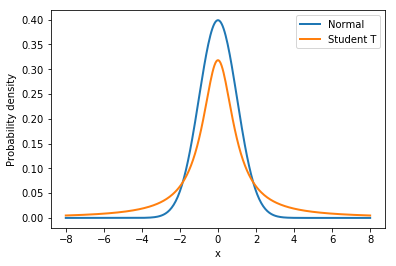
\includegraphics{images/normal_t.png}

To change the prior distribution in our PyMC3 model, we only have to
make a family and pass in to the \texttt{pm.GLM.from\_formula} function
call. The function then knows to sample from the T distribution rather
than from the normal for all the samples.

    \begin{Verbatim}[commandchars=\\\{\}]
{\color{incolor}In [{\color{incolor}25}]:} \PY{n}{formula}
\end{Verbatim}


\begin{Verbatim}[commandchars=\\\{\}]
{\color{outcolor}Out[{\color{outcolor}25}]:} 'y \textasciitilde{} failures + higher\_yes + Medu + studytime + Dalc'
\end{Verbatim}
            
    \begin{Verbatim}[commandchars=\\\{\}]
{\color{incolor}In [{\color{incolor}26}]:} \PY{n}{X\PYZus{}train\PYZus{}math}\PY{p}{[}\PY{l+s+s1}{\PYZsq{}}\PY{l+s+s1}{y}\PY{l+s+s1}{\PYZsq{}}\PY{p}{]} \PY{o}{=} \PY{n+nb}{list}\PY{p}{(}\PY{n}{y\PYZus{}train\PYZus{}math}\PY{p}{)}
         
         \PY{k}{with} \PY{n}{pm}\PY{o}{.}\PY{n}{Model}\PY{p}{(}\PY{p}{)} \PY{k}{as} \PY{n}{t\PYZus{}model}\PY{p}{:}
             \PY{n}{family} \PY{o}{=} \PY{n}{pm}\PY{o}{.}\PY{n}{glm}\PY{o}{.}\PY{n}{families}\PY{o}{.}\PY{n}{StudentT}\PY{p}{(}\PY{p}{)}
             \PY{n}{pm}\PY{o}{.}\PY{n}{GLM}\PY{o}{.}\PY{n}{from\PYZus{}formula}\PY{p}{(}\PY{n}{formula}\PY{p}{,} 
                                 \PY{n}{data} \PY{o}{=} \PY{n}{X\PYZus{}train\PYZus{}math}\PY{p}{,} \PY{n}{family} \PY{o}{=} \PY{n}{family}\PY{p}{)}
             
             \PY{c+c1}{\PYZsh{} Sample from the posterior }
             \PY{n}{t\PYZus{}trace} \PY{o}{=} \PY{n}{pm}\PY{o}{.}\PY{n}{sample}\PY{p}{(}\PY{n}{draws}\PY{o}{=}\PY{n}{NDRAWS}\PY{p}{,} \PY{n}{tune}\PY{o}{=}\PY{l+m+mi}{500}\PY{p}{,} \PY{n}{njobs} \PY{o}{=} \PY{o}{\PYZhy{}}\PY{l+m+mi}{1}\PY{p}{)}
\end{Verbatim}


    \begin{Verbatim}[commandchars=\\\{\}]
Auto-assigning NUTS sampler{\ldots}
Initializing NUTS using jitter+adapt\_diag{\ldots}
Sequential sampling (2 chains in 1 job)
NUTS: [lam\_log\_\_, Dalc, studytime, Medu, higher\_yes, failures, Intercept]
100\%|██████████| 2500/2500 [00:21<00:00, 117.44it/s]
100\%|██████████| 2500/2500 [00:17<00:00, 142.89it/s]
The acceptance probability does not match the target. It is 0.8834000488954877, but should be close to 0.8. Try to increase the number of tuning steps.

    \end{Verbatim}

    \hypertarget{investigate-trace}{%
\subsection{Investigate Trace}\label{investigate-trace}}

    \begin{Verbatim}[commandchars=\\\{\}]
{\color{incolor}In [{\color{incolor}27}]:} \PY{n}{pm}\PY{o}{.}\PY{n}{traceplot}\PY{p}{(}\PY{n}{t\PYZus{}trace}\PY{p}{)}\PY{p}{;}
\end{Verbatim}


    \begin{center}
    \adjustimage{max size={0.9\linewidth}{0.9\paperheight}}{output_52_0.png}
    \end{center}
    { \hspace*{\fill} \\}
    
    \begin{Verbatim}[commandchars=\\\{\}]
{\color{incolor}In [{\color{incolor}28}]:} \PY{n}{pm}\PY{o}{.}\PY{n}{forestplot}\PY{p}{(}\PY{n}{t\PYZus{}trace}\PY{p}{)}\PY{p}{;}
\end{Verbatim}


    \begin{center}
    \adjustimage{max size={0.9\linewidth}{0.9\paperheight}}{output_53_0.png}
    \end{center}
    { \hspace*{\fill} \\}
    
    The distributions again show the spread of each parameter sampled during
the model run. The \texttt{intercept} and \texttt{higher\_yes} variables
have the highest amount of uncertainty as was observed for the model
using a normal prior distribution.

    \hypertarget{evaluate-the-new-model}{%
\subsection{Evaluate the New Model}\label{evaluate-the-new-model}}

    \begin{Verbatim}[commandchars=\\\{\}]
{\color{incolor}In [{\color{incolor}29}]:} \PY{n}{results} \PY{o}{=} \PY{n}{evaluate\PYZus{}trace}\PY{p}{(}\PY{n}{t\PYZus{}trace}\PY{p}{,} \PY{n}{X\PYZus{}train\PYZus{}math}\PY{p}{,} \PY{n}{X\PYZus{}test\PYZus{}math}\PY{p}{,} \PY{n}{y\PYZus{}train\PYZus{}math}\PY{p}{,} \PY{n}{y\PYZus{}test\PYZus{}math}\PY{p}{,} \PY{n}{math\PYZus{}results}\PY{p}{)}
\end{Verbatim}


    \begin{Verbatim}[commandchars=\\\{\}]
Model RMSE: 2.4486
Model MAPE: 0.1330

    \end{Verbatim}

    \begin{center}
    \adjustimage{max size={0.9\linewidth}{0.9\paperheight}}{output_56_1.png}
    \end{center}
    { \hspace*{\fill} \\}
    
    \begin{center}
    \adjustimage{max size={0.9\linewidth}{0.9\paperheight}}{output_56_2.png}
    \end{center}
    { \hspace*{\fill} \\}
    
    The t-distribution metrics are nearly identical to those from the normal
distribution. As the number of samples/datapoints increases, the prior
has less and less impact on the final results because the likelihoods
come to dominate the parameters drawn from the posterior. We can do the
same querying of the new model to view the predictions for a new
student.

    \hypertarget{query-t-distribution-model}{%
\subsection{Query T-Distribution
Model}\label{query-t-distribution-model}}

    \begin{Verbatim}[commandchars=\\\{\}]
{\color{incolor}In [{\color{incolor}30}]:} \PY{n}{observation} \PY{o}{=} \PY{n}{pd}\PY{o}{.}\PY{n}{DataFrame}\PY{p}{(}\PY{p}{\PYZob{}}\PY{l+s+s1}{\PYZsq{}}\PY{l+s+s1}{Intercept}\PY{l+s+s1}{\PYZsq{}}\PY{p}{:} \PY{l+m+mi}{1}\PY{p}{,} \PY{l+s+s1}{\PYZsq{}}\PY{l+s+s1}{Medu}\PY{l+s+s1}{\PYZsq{}}\PY{p}{:} \PY{l+m+mi}{4}\PY{p}{,} \PY{l+s+s1}{\PYZsq{}}\PY{l+s+s1}{failures}\PY{l+s+s1}{\PYZsq{}}\PY{p}{:} \PY{l+m+mi}{0}\PY{p}{,} 
                                     \PY{l+s+s1}{\PYZsq{}}\PY{l+s+s1}{higher\PYZus{}yes}\PY{l+s+s1}{\PYZsq{}}\PY{p}{:} \PY{l+m+mi}{1}\PY{p}{,} \PY{l+s+s1}{\PYZsq{}}\PY{l+s+s1}{studytime}\PY{l+s+s1}{\PYZsq{}}\PY{p}{:} \PY{l+m+mi}{3}\PY{p}{,}
                                     \PY{l+s+s1}{\PYZsq{}}\PY{l+s+s1}{Dalc}\PY{l+s+s1}{\PYZsq{}}\PY{p}{:} \PY{l+m+mi}{1}\PY{p}{,} \PY{p}{\PYZcb{}}\PY{p}{,} \PY{n}{index} \PY{o}{=} \PY{p}{[}\PY{l+m+mi}{0}\PY{p}{]}\PY{p}{)}
         \PY{n}{query\PYZus{}model}\PY{p}{(}\PY{n}{t\PYZus{}trace}\PY{p}{,} \PY{n}{observation}\PY{p}{)}
\end{Verbatim}


    \begin{Verbatim}[commandchars=\\\{\}]
Average Estimate = 13.7615
5\% Estimate = 13.4020    95\% Estimate = 14.1107

    \end{Verbatim}

    \begin{center}
    \adjustimage{max size={0.9\linewidth}{0.9\paperheight}}{output_59_1.png}
    \end{center}
    { \hspace*{\fill} \\}
    
    \begin{Verbatim}[commandchars=\\\{\}]
{\color{incolor}In [{\color{incolor}31}]:} \PY{n}{observation} \PY{o}{=} \PY{n}{pd}\PY{o}{.}\PY{n}{DataFrame}\PY{p}{(}\PY{p}{\PYZob{}}\PY{l+s+s1}{\PYZsq{}}\PY{l+s+s1}{Intercept}\PY{l+s+s1}{\PYZsq{}}\PY{p}{:} \PY{l+m+mi}{1}\PY{p}{,} \PY{l+s+s1}{\PYZsq{}}\PY{l+s+s1}{Medu}\PY{l+s+s1}{\PYZsq{}}\PY{p}{:} \PY{l+m+mi}{2}\PY{p}{,} \PY{l+s+s1}{\PYZsq{}}\PY{l+s+s1}{failures}\PY{l+s+s1}{\PYZsq{}}\PY{p}{:} \PY{l+m+mi}{2}\PY{p}{,} 
                                     \PY{l+s+s1}{\PYZsq{}}\PY{l+s+s1}{higher\PYZus{}yes}\PY{l+s+s1}{\PYZsq{}}\PY{p}{:} \PY{l+m+mi}{1}\PY{p}{,} \PY{l+s+s1}{\PYZsq{}}\PY{l+s+s1}{studytime}\PY{l+s+s1}{\PYZsq{}}\PY{p}{:} \PY{l+m+mi}{2}\PY{p}{,}
                                     \PY{l+s+s1}{\PYZsq{}}\PY{l+s+s1}{Dalc}\PY{l+s+s1}{\PYZsq{}}\PY{p}{:} \PY{l+m+mi}{2}\PY{p}{,} \PY{p}{\PYZcb{}}\PY{p}{,} \PY{n}{index} \PY{o}{=} \PY{p}{[}\PY{l+m+mi}{0}\PY{p}{]}\PY{p}{)}
         \PY{n}{query\PYZus{}model}\PY{p}{(}\PY{n}{t\PYZus{}trace}\PY{p}{,} \PY{n}{observation}\PY{p}{)}
\end{Verbatim}


    \begin{Verbatim}[commandchars=\\\{\}]
Average Estimate = 9.2458
5\% Estimate = 8.6956    95\% Estimate = 9.8221

    \end{Verbatim}

    \begin{center}
    \adjustimage{max size={0.9\linewidth}{0.9\paperheight}}{output_60_1.png}
    \end{center}
    { \hspace*{\fill} \\}
    
    There is some variation between the t-distribution estimates and those
from the normal distribution as prior model. We can try other types of
prior distributions as well, but for now I will halt with the normal and
the t-distribution. Choosing appropriate priors is one of the hardest
aspect of Bayesian Modeling, but we can get around that by having more
data. As the amount of data the model learns from increases, the prior
has less of an effect because each time the posterior is updated based
on the new data. Essentially machine learning models perform inference
with no priors, basing the final model entirely on the data. In the case
of limited samples, Bayesian Inference can be a better method for
building models because it provides a reasonable estimate in situations
with few data points (as long as the prior is reasonable).

    \hypertarget{conclusions}{%
\section{Conclusions}\label{conclusions}}

In this notebook we looked at using Bayesian Linear Regression to
predict student performance based on five factors. Rather than specify
probabilities for the Bayesian network which is basically impossible for
continuous variables, we framed the problem as a machine learning task.
In addition to the standard machine learning models that learn from
observations, we also used Bayesian Linear Regression to create a model
mapping the features (student characteristics) to the targets (final
grade). The advantages of Bayesian Linear Regression are that if we use
sensible priors, we can still get a decent estimate with few samples,
and the final weights are not a single number, but a distribution
componsed of every sample drawn during the sampling run. We can then
make predictions using all the sampled weights to form a distribution of
expected values rather than a single answer.

The Bayesian Linear Regression did not perform as well as the other
methods in terms of the two metrics we choose. This might not be the
ideal case for a Bayesian inference approach but we saw that Bayesian
Linear Regression produced intuitive estimates for the model weights and
gave predictions for new students that align with our expectations for
the factors influencing student performance. To summarize, although
Bayesian Linear Regression did not outperform the standard machine
learning methods, it gave us a chance to learn another tool for use in
evaluation and making sense of data. There are likely situations in
which Bayesian inference is better suited than standard machine
learning, and it is best to be prepared for those situations when we
find them.


    % Add a bibliography block to the postdoc
    
    
    
    \end{document}
